\documentclass[12pt, a4paper]{report}

% ══════════════════════════════════════════════════════════════
%  PACKAGES
% ══════════════════════════════════════════════════════════════
\usepackage[utf8]{inputenc}
\usepackage[T1]{fontenc}
\usepackage[portuguese]{babel}
\usepackage{lmodern}
\usepackage{microtype}

\usepackage[
  a4paper,
  top=2.8cm, bottom=2.8cm,
  left=3cm,  right=2.5cm
]{geometry}

\usepackage[table]{xcolor}
\usepackage{graphicx}
\usepackage{booktabs}
\usepackage{tabularx}
\usepackage{multirow}
\usepackage{longtable}
\usepackage{array}
\usepackage{fancyhdr}
\usepackage{titlesec}
\usepackage{titletoc}
\usepackage{tcolorbox}
\usepackage{listings}
\usepackage{enumitem}
\usepackage{parskip}
\usepackage{float}
\usepackage{caption}
\usepackage{setspace}
\usepackage{hyperref}
\usepackage{tikz}
\usepackage{pgf}
\usetikzlibrary{shapes.geometric, arrows.meta, positioning, fit, backgrounds, calc}

\tcbuselibrary{skins, breakable}
\renewcommand{\arraystretch}{1.3}


% ══════════════════════════════════════════════════════════════
%  CORES
% ══════════════════════════════════════════════════════════════
\definecolor{NavyBlue}  {RGB}{20,  50,  100}
\definecolor{MidBlue}   {RGB}{40,  80,  140}
\definecolor{LightBlue} {RGB}{230, 237, 248}
\definecolor{TableHead} {RGB}{35,  60,  110}
\definecolor{TableAlt}  {RGB}{245, 247, 251}
\definecolor{LineGray}  {RGB}{180, 185, 195}
\definecolor{TextGray}  {RGB}{90,  95,  105}

\definecolor{Critical}  {RGB}{180, 30,  30}
\definecolor{High}      {RGB}{200, 85,  20}
\definecolor{Medium}    {RGB}{190, 145, 0}
\definecolor{Low}       {RGB}{50,  140, 70}

\definecolor{CodeBg}    {RGB}{245, 246, 248}
\definecolor{CodeFrame} {RGB}{210, 215, 225}

% Cores para o diagrama TikZ
\definecolor{DMZColor}      {RGB}{255, 200, 100}
\definecolor{ServerColor}   {RGB}{180, 210, 255}
\definecolor{UserColor}     {RGB}{180, 230, 180}
\definecolor{FWColor}       {RGB}{220, 80,  60}
\definecolor{InternetColor} {RGB}{200, 200, 200}


% ══════════════════════════════════════════════════════════════
%  HYPERREF
% ══════════════════════════════════════════════════════════════
\hypersetup{
  colorlinks = true,
  linkcolor  = NavyBlue,
  urlcolor   = MidBlue,
  pdftitle   = {Relatorio de Auditoria de Seguranca -- HealthIT},
  pdfauthor  = {[Nome do Aluno]},
}


% ══════════════════════════════════════════════════════════════
%  CABECALHO / RODAPE
% ══════════════════════════════════════════════════════════════
\pagestyle{fancy}
\fancyhf{}
\fancyhead[L]{\small\color{TextGray}Auditoria de Seguranca -- HealthIT}
\fancyhead[R]{\small\color{TextGray}LSIRC \textperiodcentered{} 2025/2026}
\fancyfoot[C]{\small\color{TextGray}\thepage}
\renewcommand{\headrulewidth}{0.4pt}
\renewcommand{\headrule}{\color{LineGray}\hrule height 0.4pt}

\fancypagestyle{plain}{
  \fancyhf{}
  \fancyfoot[C]{\small\color{TextGray}\thepage}
  \renewcommand{\headrulewidth}{0pt}
}


% ══════════════════════════════════════════════════════════════
%  TITULOS
% ══════════════════════════════════════════════════════════════
\titleformat{\chapter}[block]
  {\Large\bfseries\color{NavyBlue}}
  {\thechapter.}{0.6em}{}
  [\vspace{2pt}{\color{NavyBlue}\rule{\linewidth}{1.2pt}}]

\titlespacing{\chapter}{0pt}{0pt}{16pt}

\titleformat{\section}
  {\large\bfseries\color{NavyBlue}}
  {\thesection}{0.6em}{}

\titlespacing{\section}{0pt}{14pt}{4pt}

\titleformat{\subsection}
  {\normalsize\bfseries\color{MidBlue}}
  {\thesubsection}{0.6em}{}

\titlespacing{\subsection}{0pt}{10pt}{2pt}


% ══════════════════════════════════════════════════════════════
%  CODIGO
% ══════════════════════════════════════════════════════════════
\lstset{
  backgroundcolor = \color{CodeBg},
  basicstyle      = \ttfamily\small,
  breaklines      = true,
  frame           = single,
  rulecolor       = \color{CodeFrame},
  numbers         = left,
  numberstyle     = \tiny\color{TextGray},
  numbersep       = 8pt,
  showstringspaces= false,
  tabsize         = 2,
  captionpos      = b,
  xleftmargin     = 12pt,
  xrightmargin    = 4pt,
}


% ══════════════════════════════════════════════════════════════
%  CAIXAS
% ══════════════════════════════════════════════════════════════
\newtcolorbox{notebox}{
  colback  = LightBlue,
  colframe = MidBlue,
  boxrule  = 0.5pt,
  arc      = 2pt,
  left=8pt, right=8pt, top=6pt, bottom=6pt,
  fontupper= \small,
}

\newtcolorbox{alertbox}{
  colback  = Critical!8,
  colframe = Critical!60,
  boxrule  = 0.5pt,
  arc      = 2pt,
  left=8pt, right=8pt, top=6pt, bottom=6pt,
  fontupper= \small,
}

\newtcolorbox{finding}[1]{
  colback  = white,
  colframe = LineGray,
  boxrule  = 0.5pt,
  arc      = 2pt,
  left=10pt, right=8pt, top=8pt, bottom=8pt,
  title    = {\small\bfseries #1},
  coltitle = white,
  attach boxed title to top left = {yshift=-0.5mm, xshift=4pt},
  boxed title style = {
    colback=NavyBlue, colframe=NavyBlue,
    arc=2pt, boxrule=0pt,
    top=3pt, bottom=3pt, left=6pt, right=6pt,
  },
  breakable,
}


% ══════════════════════════════════════════════════════════════
%  COMANDOS AUXILIARES
% ══════════════════════════════════════════════════════════════
\newcommand{\risk}[1]{%
  \ifnum\pdfstrcmp{#1}{Critico}=0{\colorbox{Critical}{\color{white}\bfseries\footnotesize\strut~Critico~}}\fi
  \ifnum\pdfstrcmp{#1}{Alto}=0{\colorbox{High}{\color{white}\bfseries\footnotesize\strut~Alto~}}\fi
  \ifnum\pdfstrcmp{#1}{Medio}=0{\colorbox{Medium}{\color{black}\bfseries\footnotesize\strut~Medio~}}\fi
  \ifnum\pdfstrcmp{#1}{Baixo}=0{\colorbox{Low}{\color{white}\bfseries\footnotesize\strut~Baixo~}}\fi
}

\newcommand{\thead}[1]{\bfseries\small\color{white}#1}


% ══════════════════════════════════════════════════════════════
\begin{document}
\setstretch{1.15}


% ──────────────────────────────────────────────────────────────
%  CAPA
% ──────────────────────────────────────────────────────────────
\begin{titlepage}
\centering

\vspace*{2cm}

{\color{NavyBlue}\rule{\linewidth}{2pt}}
\vspace{0.3cm}
{\color{NavyBlue}\rule{\linewidth}{0.4pt}}

\vspace{1.5cm}

{\LARGE\bfseries\color{NavyBlue} Relatorio de Auditoria de Seguranca}

\vspace{0.4cm}

{\large\color{TextGray} Empresa HealthIT}

\vspace{1.5cm}

{\color{NavyBlue}\rule{0.5\linewidth}{0.4pt}}

\vspace{1.5cm}

\begin{tabular}{rl}
  \textbf{Instituicao}       & Instituto Politecnico do Porto -- ESTGF \\[5pt]
  \textbf{Licenciatura}      & LSIRC \\[5pt]
  \textbf{Unidade Curricular}& Auditoria Informatica \\[5pt]
  \textbf{Docente}           & Alfredo Franca \\[5pt]
  \textbf{Aluno}             & \textit{[Nome Completo]} \\[5pt]   % PREENCHER
  \textbf{Numero}            & \textit{[Numero de Aluno]} \\[5pt] % PREENCHER
  \textbf{Ano Letivo}        & 2025/2026 \\[5pt]
  \textbf{Data de Entrega}   & 28 de Abril de 2026 \\
\end{tabular}

\vfill

{\color{NavyBlue}\rule{0.5\linewidth}{0.4pt}}

\vspace{0.5cm}

{\small\color{TextGray}\textit{Documento confidencial -- distribuicao restrita}}

\vspace{0.4cm}

{\color{NavyBlue}\rule{\linewidth}{0.4pt}}
\vspace{0.1cm}
{\color{NavyBlue}\rule{\linewidth}{2pt}}

\end{titlepage}


% ──────────────────────────────────────────────────────────────
%  INDICE
% ──────────────────────────────────────────────────────────────
\tableofcontents
\newpage


% ══════════════════════════════════════════════════════════════
\chapter{Sumario Executivo}
% ══════════════════════════════════════════════════════════════

Este relatorio apresenta os resultados da auditoria de seguranca
realizada a infraestrutura de TI da empresa \textbf{HealthIT}, no
ambito da unidade curricular de Auditoria Informatica da Licenciatura
em Seguranca Informatica de Redes e Computadores (LSIRC), ano letivo
2025/2026.

A auditoria incidiu sobre a rede interna \texttt{192.168.50.0/24},
abrangendo tres ativos principais: o Windows Server 2019 (controlador
de dominio e servidor de ficheiros), o Ubuntu Server 22.04 (servidor
web, API e base de dados clinica) e o Windows 10 (estacao de trabalho
cliente). A maquina Kali Linux foi utilizada como plataforma de auditoria
e nao e considerada ativo da empresa.

Foram identificadas \textbf{9 vulnerabilidades} no total, distribuidas
da seguinte forma:

\begin{table}[H]
\centering
\begin{tabular}{l c}
\toprule
\rowcolor{TableHead}
\thead{Nivel de Risco} & \thead{Quantidade} \\
\midrule
\risk{Critico} & 4 \\
\rowcolor{TableAlt}
\risk{Alto}    & 4 \\
\risk{Medio}   & 1 \\
\rowcolor{TableAlt}
\risk{Baixo}   & 0 \\
\midrule
\textbf{Total} & \textbf{9} \\
\bottomrule
\end{tabular}
\end{table}

O ativo mais critico identificado e o \textbf{Ubuntu Server 22.04}
(192.168.50.30), que aloja a aplicacao web clinica e a base de dados
com registos de pacientes. A vulnerabilidade de \textbf{SQL Injection}
encontrada neste servidor permite extrair dados clinicos sem qualquer
autenticacao, o que constitui uma violacao direta do RGPD, nomeadamente
do Artigo 9.o (categorias especiais de dados).

Outro achado particularmente grave foi a existencia do ficheiro
\texttt{HealthIT\_passwords.xlsx} numa partilha de rede acessivel
com as credenciais comprometidas encontradas na \textit{dark web}.
Este ficheiro contem as passwords de toda a infraestrutura em texto
claro e, por si so, seria suficiente para um atacante comprometer
simultaneamente todos os sistemas da empresa.

A empresa foi notificada pelo Centro Nacional de Ciberseguranca (CNCS)
da existencia de credenciais comprometidas na \textit{dark web}
(\texttt{joao / Password1}). A validade destas credenciais foi
confirmada durante a auditoria, com acesso a partilhas sensiveis,
dados financeiros e dados pessoais de clientes.

\textbf{Nivel de maturidade de seguranca (escala 1 a 5): 1 -- Inicial.}
A empresa nao tem processos formais de seguranca definidos, a gestao de
credenciais e feita de forma ad hoc e a infraestrutura nao esta segmentada.

Dada a restricao operacional de \textbf{5 correcoes em 3 meses},
foram priorizadas as seguintes vulnerabilidades:

\begin{enumerate}[leftmargin=*, itemsep=2pt]
  \item \textbf{VUL-01} -- Revogacao imediata das credenciais
        comprometidas e implementacao de MFA
  \item \textbf{VUL-03} -- Correcao da SQL Injection na aplicacao
        web clinica
  \item \textbf{VUL-02} -- Eliminacao do ficheiro de passwords
        e implementacao de gestor de passwords empresarial
  \item \textbf{VUL-09} -- Implementacao de segmentacao de rede
        com VLANs e firewall interno
  \item \textbf{VUL-05} -- Implementacao de politica de passwords
        forte com lockout e MFA no dominio
\end{enumerate}

A implementacao destas medidas reduzira de forma significativa a
exposicao da HealthIT a ataques e contribuira para a conformidade
com o RGPD, o que e um requisito fundamental para a adjudicacao
do contrato hospitalar em negociacao.


% ══════════════════════════════════════════════════════════════
\chapter{Enquadramento}
% ══════════════════════════════════════════════════════════════

A empresa \textbf{HealthIT} desenvolve e mantem uma plataforma web
de gestao clinica utilizada por clinicas privadas e unidades hospitalares.
Estando em fase de negociacao de um contrato com uma nova entidade
hospitalar, foi exigida a realizacao de uma auditoria de seguranca como
requisito previo a adjudicacao.

O objetivo desta auditoria nao se limita apenas a identificar
vulnerabilidades tecnicas. Pretende-se tambem avaliar o risco real
para o negocio, tendo em conta o tipo de dados processados, o impacto
legal e financeiro de um eventual incidente e a necessidade de priorizar
as medidas corretivas face as restricoes operacionais existentes.

\section{Ambito}

A auditoria incidiu sobre a rede interna \texttt{192.168.50.0/24},
abrangendo todos os ativos presentes. A plataforma de auditoria utilizada
foi exclusivamente a maquina Kali Linux (\texttt{192.168.50.10}). Nao
foram realizadas quaisquer acoes destrutivas sobre os sistemas auditados.

\section{Restricoes Operacionais}

\begin{notebox}
A empresa tem recursos para corrigir apenas \textbf{5 vulnerabilidades}
nos proximos 3 meses. A selecao e priorizacao dessas vulnerabilidades
e um dos produtos centrais deste relatorio.
\end{notebox}

\vspace{0.6em}

\begin{alertbox}
O Centro Nacional de Ciberseguranca notificou a empresa da existencia
de credenciais comprometidas na \textit{dark web}:\\
\texttt{User: joao \quad Password: Password1}\\
A validade e o alcance destas credenciais foram verificados no decurso
da auditoria.
\end{alertbox}


% ══════════════════════════════════════════════════════════════
\chapter{Arquitetura e Ativos}
% ══════════════════════════════════════════════════════════════

\section{Topologia de Rede}

A infraestrutura opera numa rede interna plana (\texttt{192.168.50.0/24}),
sem qualquer segmentacao entre zonas de servidores e estacoes de trabalho.
O gateway \texttt{192.168.50.1} serve apenas para simular acesso a Internet.
Esta ausencia de segmentacao e, por si so, um vetor de risco significativo,
pois qualquer maquina comprometida tem acesso direto a todos os outros
sistemas da rede.

\section{Inventario de Maquinas}

\begin{table}[H]
\centering
\caption{Inventario de Ativos}
\begin{tabularx}{\linewidth}{>{\ttfamily}c l X}
\toprule
\rowcolor{TableHead}
\thead{Endereco IP} & \thead{Maquina} & \thead{Funcoes} \\
\midrule
192.168.50.10 & Kali Linux          & Plataforma de auditoria \\
\rowcolor{TableAlt}
192.168.50.20 & Windows Server 2019 & Active Directory, DNS, Servidor de Ficheiros (SMB) \\
192.168.50.30 & Ubuntu Server 22.04 & Servidor Web, API, Base de Dados MySQL \\
\rowcolor{TableAlt}
192.168.50.40 & Windows 10          & Estacao de trabalho, cliente de dominio \\
\bottomrule
\end{tabularx}
\end{table}

\section{Classificacao de Ativos}

A tabela seguinte apresenta a classificacao de cada ativo de acordo
com a criticidade para o negocio, tendo em conta a informacao que
processa e o impacto de um eventual compromisso.

\begin{table}[H]
\centering
\caption{Classificacao de Ativos por Criticidade}
\begin{tabularx}{\linewidth}{l l X c X}
\toprule
\rowcolor{TableHead}
\thead{Ativo} & \thead{Tipo} & \thead{Informacao Processada}
  & \thead{Criticidade} & \thead{Justificacao} \\
\midrule
Ubuntu Server 22.04
  & Servidor
  & Dados clinicos, dados pessoais (RGPD), backups da BD
  & \risk{Critico}
  & Aloja a BD clinica com dados de saude de pacientes (categorias especiais
    RGPD, Artigo 9.o). Um compromisso implica violacao legal imediata e perda
    do contrato hospitalar. \\
\rowcolor{TableAlt}
Windows Server 2019
  & Servidor
  & Credenciais AD, informacao financeira, documentacao interna
  & \risk{Critico}
  & Controlador de dominio -- um compromisso total permite acesso a toda a
    infraestrutura. Contem tambem dados financeiros de clientes com dados
    bancarios (IBAN, NIF). \\
Windows 10
  & Workstation
  & Credenciais em cache, sessoes AD, ficheiros exportados
  & \risk{Alto}
  & Ponto de entrada potencial para movimento lateral. Tem acesso autenticado
    ao dominio e a partilhas sensiveis. \\
\rowcolor{TableAlt}
Kali Linux
  & Auditor
  & Sem dados da empresa
  & \risk{Baixo}
  & Maquina do auditor, utilizada exclusivamente para testes. Nao armazena
    dados da empresa. \\
\bottomrule
\end{tabularx}
\end{table}


% ══════════════════════════════════════════════════════════════
\chapter{Metodologia}
% ══════════════════════════════════════════════════════════════

A auditoria seguiu uma abordagem faseada baseada no \textbf{PTES}
(\textit{Penetration Testing Execution Standard}) e na
\textbf{OWASP Testing Guide v4.2}. O PTES foi escolhido por fornecer
uma estrutura clara para cada fase do processo de auditoria, desde o
reconhecimento inicial ate ao reporte final. A OWASP Testing Guide
foi utilizada especificamente para guiar os testes a aplicacao web
clinica, dado que define metodologias concretas para testar
vulnerabilidades como SQL Injection e XSS em aplicacoes web.

As fases seguidas foram as seguintes:

\begin{enumerate}[leftmargin=*, itemsep=4pt]
  \item \textbf{Reconhecimento passivo} -- analise da notificacao
        do CNCS relativa as credenciais comprometidas na \textit{dark web},
        identificando o utilizador e a password expostos como ponto de
        partida da auditoria;
  \item \textbf{Descoberta de ativos} -- varrimento da rede interna
        com arp-scan e Nmap para identificar todos os hosts ativos;
  \item \textbf{Enumeracao de servicos} -- identificacao de portas abertas,
        versoes de software e servicos expostos em cada ativo;
  \item \textbf{Analise de vulnerabilidades} -- utilizacao de ferramentas
        automatizadas (Nessus, Nuclei) para identificar vulnerabilidades
        conhecidas, complementadas com testes manuais;
  \item \textbf{Validacao e prova de conceito} -- confirmacao manual das
        vulnerabilidades identificadas, sem realizar acoes destrutivas
        sobre os sistemas;
  \item \textbf{Analise de trafego} -- captura de trafego de rede com
        Wireshark para identificar comunicacoes sem cifra e credenciais
        expostas;
  \item \textbf{Avaliacao de risco} -- classificacao de cada finding
        por Probabilidade de Exploracao e Impacto no Negocio;
  \item \textbf{Reporte} -- documentacao de todas as evidencias e
        elaboracao de recomendacoes priorizadas.
\end{enumerate}

\textbf{Limitacoes da abordagem:} A auditoria foi realizada num
ambiente de laboratorio controlado, sem acesso a Internet real. Nao
foram testados vetores de ataque externos (como engenharia social ou
ataques de phishing). Os testes foram realizados sem conhecimento
previo da infraestrutura (abordagem \textit{black box} parcial),
com excecao das credenciais fornecidas pelo CNCS.

\section{Ferramentas Utilizadas}

\begin{table}[H]
\centering
\caption{Ferramentas de Auditoria}
\begin{tabularx}{\linewidth}{l X}
\toprule
\rowcolor{TableHead}
\thead{Ferramenta} & \thead{Finalidade} \\
\midrule
Nmap / arp-scan  & Descoberta de hosts e varrimento de portas e servicos \\
\rowcolor{TableAlt}
Nessus Essentials & Analise automatizada de vulnerabilidades nos servidores \\
Nuclei           & Deteção de vulnerabilidades em aplicacoes web \\
\rowcolor{TableAlt}
Wireshark        & Captura e analise de trafego de rede \\
smbclient        & Enumeracao e acesso a partilhas SMB \\
\rowcolor{TableAlt}
enum4linux       & Enumeracao do dominio Active Directory \\
Bloodhound       & Analise de caminhos de ataque no Active Directory \\
\rowcolor{TableAlt}
sqlmap           & Deteção e validacao de SQL Injection \\
\bottomrule
\end{tabularx}
\end{table}


% ══════════════════════════════════════════════════════════════
\chapter{Resultados Tecnicos}
% ══════════════════════════════════════════════════════════════

% ──────────────────────────────────────────────────────────────
\section{Reconhecimento Passivo}
% ──────────────────────────────────────────────────────────────

O ponto de partida desta auditoria foi a notificacao recebida pelo
Centro Nacional de Ciberseguranca (CNCS), que alertou para a existencia
de credenciais da empresa HealthIT expostas numa plataforma da
\textit{dark web}. As credenciais identificadas foram:

\begin{center}
\texttt{Utilizador: joao \quad Password: Password1}
\end{center}

Antes de iniciar qualquer varrimento ativo, foi feita uma analise
desta notificacao para perceber o alcance potencial do compromisso.
Verificou-se que:

\begin{itemize}[itemsep=2pt]
  \item A password \texttt{Password1} e extremamente fraca e e
        uma das primeiras a ser testada em ataques de dicionario;
  \item O nome de utilizador \texttt{joao} e um nome comum em
        dominios portugueses, o que sugere uma conta de utilizador
        real e nao uma conta de servico;
  \item A exposicao na \textit{dark web} indica que estas
        credenciais podem ja estar a ser exploradas por terceiros
        maliciosos, pelo que a situacao exige resposta imediata.
\end{itemize}

Esta fase orientou toda a estrategia de auditoria seguinte, com
foco inicial na validacao das credenciais e na avaliacao do seu
alcance na infraestrutura da empresa.

% ──────────────────────────────────────────────────────────────
\section{Descoberta de Hosts}
% ──────────────────────────────────────────────────────────────

Para identificar todos os hosts ativos na rede interna, foi executado
o seguinte comando a partir da maquina de auditoria (Kali Linux,
\texttt{192.168.50.10}):

\begin{lstlisting}[language=bash, caption={Comando de descoberta de hosts}]
sudo arp-scan -I enp0s8 192.168.50.0/24
\end{lstlisting}

\begin{figure}[H]
  \centering
  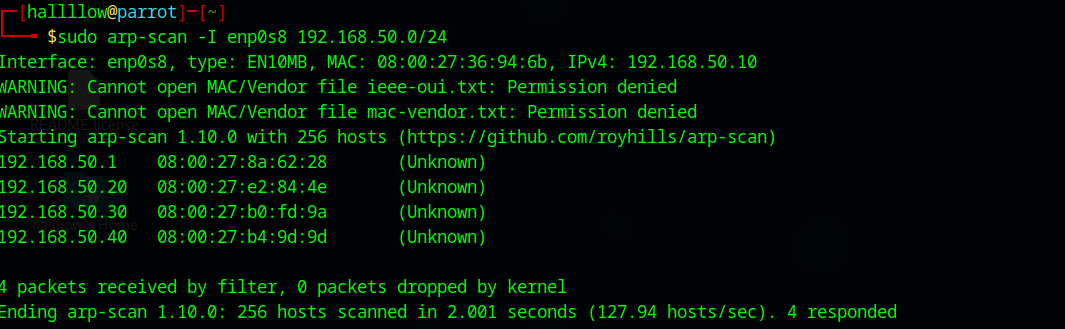
\includegraphics[width=\linewidth]{images/scan_inicial.png}
  \caption{Resultado da descoberta de hosts na rede 192.168.50.0/24}
  \label{fig:scan_inicial}
\end{figure}

Os resultados confirmam a presenca dos quatro ativos esperados na
rede interna, todos acessiveis a partir da maquina de auditoria
sem qualquer restricao de firewall entre segmentos.

% ──────────────────────────────────────────────────────────────
\section{Enumeracao de Servicos}
% ──────────────────────────────────────────────────────────────

Apos confirmar quais os hosts ativos, procedeu-se a enumeracao
detalhada dos servicos em execucao em cada ativo, com o objetivo
de identificar portas abertas, versoes de software e possiveis
vetores de ataque.

\newpage
\subsection{Windows Server 2019 -- 192.168.50.20}

\begin{lstlisting}[language=bash, caption={Nmap -- 192.168.50.20}]
sudo nmap -Pn -sS -sV -sC 192.168.50.20
\end{lstlisting}

\begin{figure}[H]
  \centering
  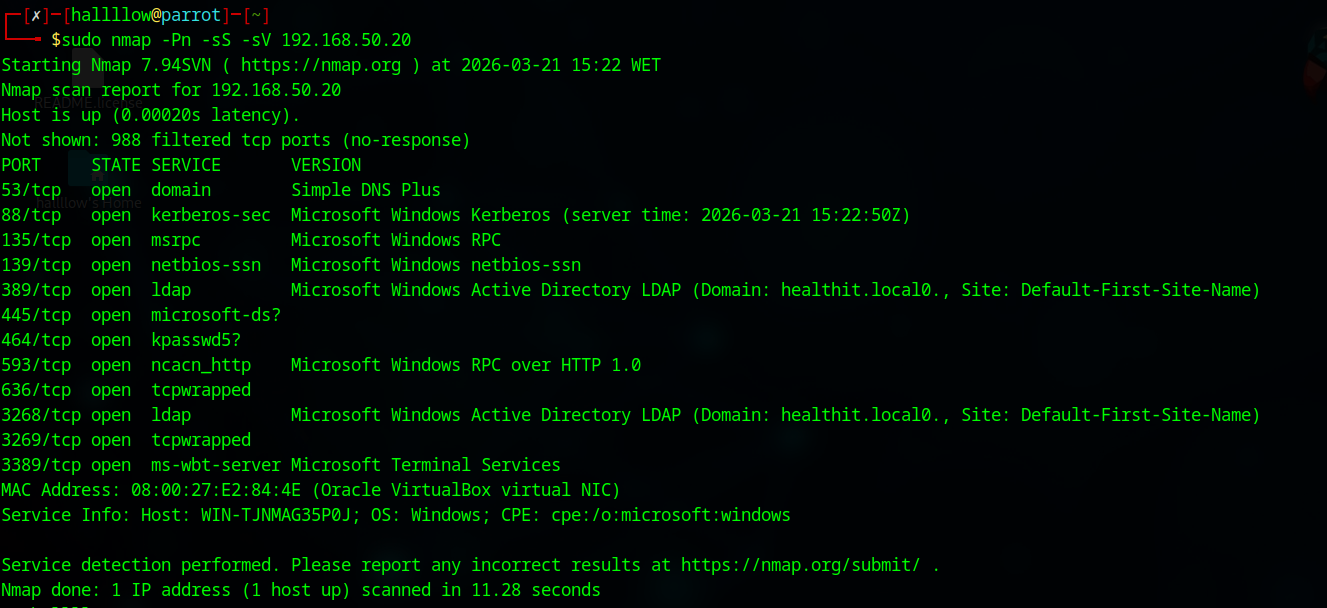
\includegraphics[width=\linewidth]{images/windows_scan.png}
  \caption{Resultado da enumeracao do Windows Server 2019}
  \label{fig:scan_winserver}
\end{figure}

\begin{table}[H]
\centering
\caption{Portas e Servicos -- 192.168.50.20}
\begin{tabularx}{\linewidth}{c c l X}
\toprule
\rowcolor{TableHead}
\thead{Porta} & \thead{Proto.} & \thead{Servico} & \thead{Observacao} \\
\midrule
53   & TCP & DNS         & Simple DNS Plus -- Active Directory DNS \\
\rowcolor{TableAlt}
88   & TCP & Kerberos    & Autenticacao de dominio (\texttt{healthit.local}) \\
135  & TCP & RPC         & Microsoft Windows RPC \\
\rowcolor{TableAlt}
139  & TCP & NetBIOS     & Microsoft NetBIOS-SSN \\
389  & TCP & LDAP        & Active Directory -- dominio \texttt{healthit.local} \\
\rowcolor{TableAlt}
445  & TCP & SMB         & Microsoft Directory Services \\
464  & TCP & kpasswd     & Kerberos -- alteracao de passwords \\
\rowcolor{TableAlt}
593  & TCP & RPC/HTTP    & Microsoft RPC over HTTP 1.0 \\
3268 & TCP & LDAP        & Global Catalog Active Directory \\
\rowcolor{TableAlt}
3389 & TCP & RDP         & Terminal Services -- acesso remoto exposto \\
\bottomrule
\end{tabularx}
\end{table}

De notar que o servico RDP (porta 3389) esta exposto a toda a rede
interna sem qualquer restricao. Isto significa que qualquer maquina
comprometida na rede pode tentar autenticar-se remotamente no servidor,
o que aumenta significativamente a superficie de ataque.

\newpage
\subsection{Enumeracao de Partilhas SMB}

Com as credenciais obtidas na fase de reconhecimento passivo, foi
feita a enumeracao das partilhas SMB disponiveis no servidor:

\begin{lstlisting}[language=bash, caption={Enumeracao de partilhas SMB}]
smbclient -L //192.168.50.20 -U joao%Password1
\end{lstlisting}

\begin{figure}[H]
  \centering
  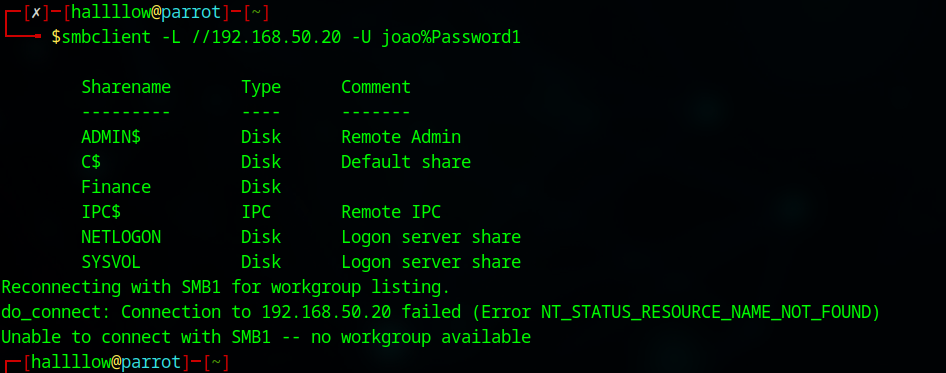
\includegraphics[width=\linewidth]{images/smblcient_enum.png}
  \caption{Partilhas SMB accessiveis com as credenciais comprometidas}
  \label{fig:smbclient_enum}
\end{figure}

Os resultados mostram que o utilizador \texttt{joao} tem acesso a
partilhas de elevada sensibilidade, incluindo partilhas administrativas
que nao deviam ser acessiveis a contas comuns:

\begin{table}[H]
\centering
\caption{Partilhas SMB Accessiveis -- 192.168.50.20}
\begin{tabularx}{\linewidth}{l l X c}
\toprule
\rowcolor{TableHead}
\thead{Partilha} & \thead{Tipo} & \thead{Observacao} & \thead{Risco} \\
\midrule
\texttt{ADMIN\$}   & Disk & Acesso administrativo remoto ao sistema & \risk{Critico} \\
\rowcolor{TableAlt}
\texttt{C\$}       & Disk & Acesso total ao disco do servidor & \risk{Critico} \\
\texttt{Finance}   & Disk & Informacao financeira sensivel da empresa & \risk{Critico} \\
\rowcolor{TableAlt}
\texttt{NETLOGON}  & Disk & Scripts de logon do dominio & \risk{Alto} \\
\texttt{SYSVOL}    & Disk & Politicas de grupo do Active Directory & \risk{Alto} \\
\rowcolor{TableAlt}
\texttt{IPC\$}     & IPC  & Canal de comunicacao entre processos & \risk{Medio} \\
\bottomrule
\end{tabularx}
\end{table}

O acesso as partilhas \texttt{ADMIN\$} e \texttt{C\$} com credenciais
de um utilizador comum indica uma configuracao de privilegios excessivos.
Foi tambem detetada a utilizacao do protocolo \textbf{SMBv1}, considerado
obsoleto e vulneravel a ataques como o \textit{EternalBlue}, responsavel
pela propagacao do ransomware WannaCry.

\newpage
\subsection{Acesso e Analise da Partilha Finance}

Foi feito o acesso direto a partilha \texttt{Finance} para listar
e transferir os ficheiros disponiveis:

\begin{lstlisting}[language=bash, caption={Acesso a partilha Finance e extracao de ficheiros}]
smbclient //192.168.50.20/Finance -U joao%Password1
smb:\> dir
smb:\> get HealthIT_Dados_Financeiros_Clientes_v2.xlsx
smb:\> get HealthIT_passwords.xlsx
\end{lstlisting}

\begin{figure}[H]
  \centering
  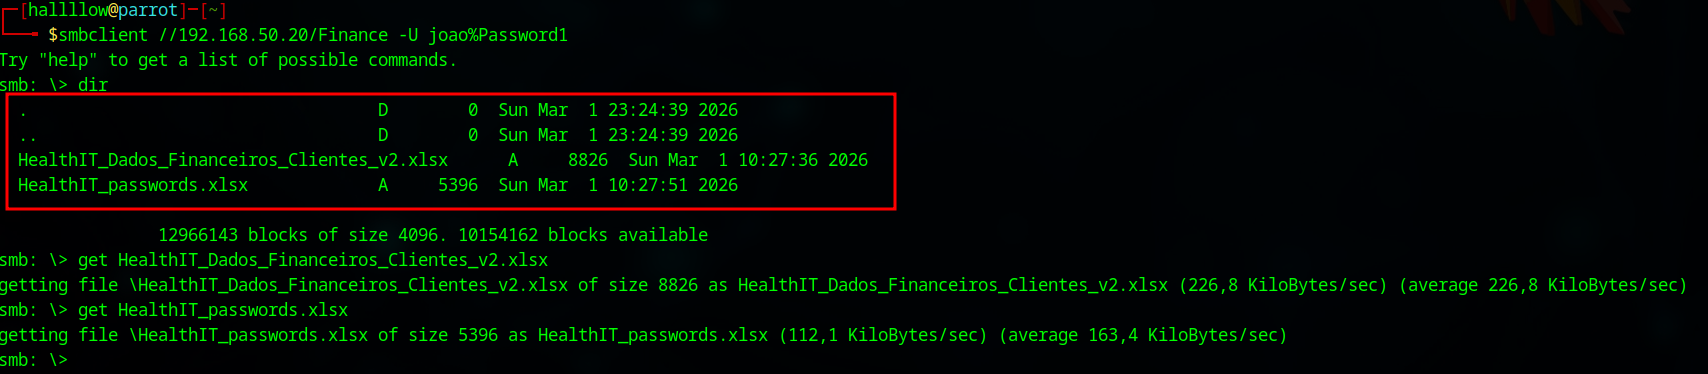
\includegraphics[width=\linewidth]{images/smbclient_finance.png}
  \caption{Listagem e extracao de ficheiros da partilha Finance}
  \label{fig:smbclient_finance}
\end{figure}

Foram identificados e transferidos dois ficheiros de elevada
sensibilidade.

\newpage
\subsubsection{HealthIT\_Dados\_Financeiros\_Clientes\_v2.xlsx}

A analise deste ficheiro revelou a exposicao de informacao de
identificacao pessoal (PII) de clientes, em violacao direta do
RGPD (Artigo 5.o, principio da integridade e confidencialidade,
e Artigo 32.o, seguranca do tratamento):

\begin{lstlisting}[language=bash, caption={Extracao do conteudo do ficheiro financeiro}]
xlsx2csv HealthIT_Dados_Financeiros_Clientes_v2.xlsx
\end{lstlisting}

\begin{figure}[H]
  \centering
  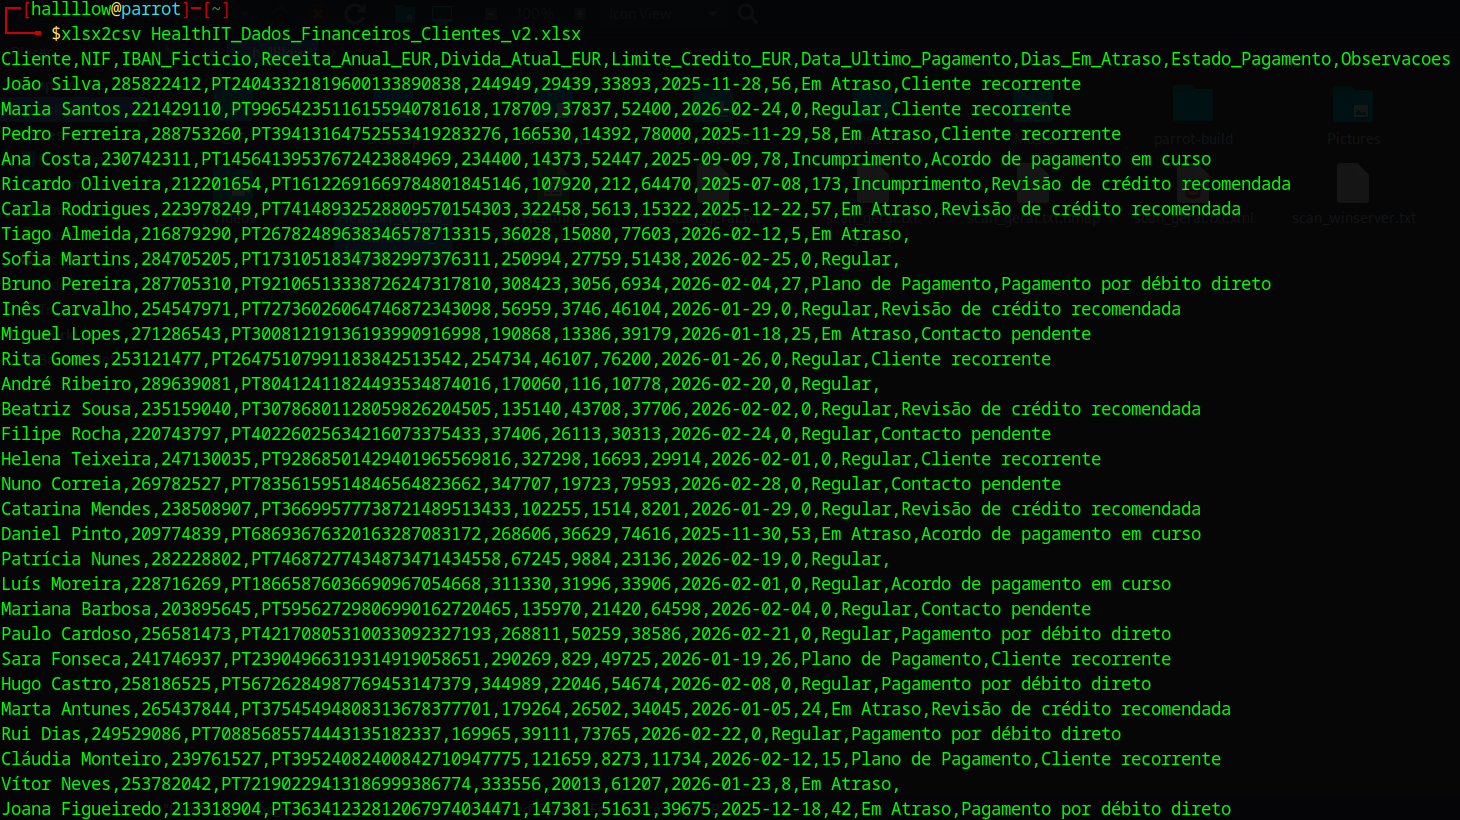
\includegraphics[width=\linewidth]{images/healthIt_dados_finance.png}
  \caption{Dados financeiros e PII expostos na partilha Finance}
  \label{fig:dados_financeiros}
\end{figure}

Os dados expostos incluem, para cada cliente:

\begin{itemize}[itemsep=2pt]
  \item \textbf{Nome completo}
  \item \textbf{NIF} -- numero de identificacao fiscal
  \item \textbf{IBAN} -- dados bancarios completos
  \item \textbf{Receita anual e divida atual} em euros
  \item \textbf{Estado de pagamento} e datas de incumprimento
\end{itemize}

A exposicao deste ficheiro numa partilha acessivel com credenciais
comuns constitui uma violacao grave do RGPD, podendo resultar em
multas ate \textbf{4\% do volume de negocios anual} da empresa.

\newpage
\subsubsection{HealthIT\_passwords.xlsx}

O segundo ficheiro e ainda mais grave. Trata-se de um repositorio
de credenciais de acesso a multiplos sistemas da empresa, armazenado
de forma completamente insegura numa partilha de rede partilhada:

\begin{lstlisting}[language=bash, caption={Extracao do conteudo do ficheiro de passwords}]
xlsx2csv HealthIT_passwords.xlsx
\end{lstlisting}

\begin{figure}[H]
  \centering
  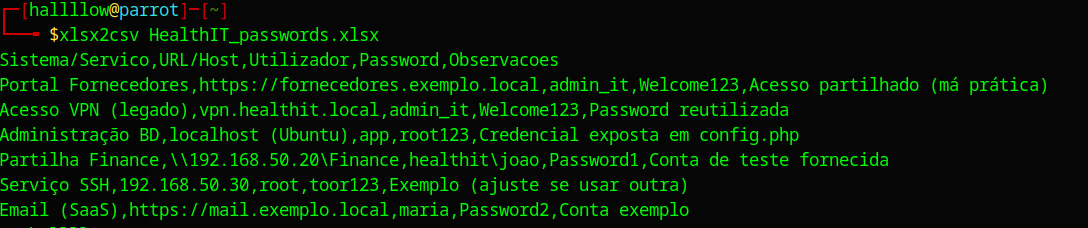
\includegraphics[width=\linewidth]{images/HealthIT_passwords.png}
  \caption{Ficheiro de credenciais exposto na partilha Finance}
  \label{fig:passwords_xlsx}
\end{figure}

\begin{table}[H]
\centering
\caption{Credenciais Expostas no Ficheiro HealthIT\_passwords.xlsx}
\begin{tabularx}{\linewidth}{l l l X}
\toprule
\rowcolor{TableHead}
\thead{Sistema/Servico} & \thead{Utilizador} & \thead{Password} & \thead{Observacao} \\
\midrule
Portal Fornecedores   & admin\_it  & Welcome123  & Acesso partilhado, ma pratica \\
\rowcolor{TableAlt}
Acesso VPN (legado)   & admin\_it  & Welcome123  & Password reutilizada \\
Administracao BD (Ubuntu) & app    & root123     & Credencial exposta em config.php \\
\rowcolor{TableAlt}
Partilha Finance      & healthit\textbackslash joao & Password1 & Conta comprometida \\
Servico SSH           & root       & toor123     & Acesso root direto ao Ubuntu \\
\rowcolor{TableAlt}
Email (SaaS)          & maria      & Password2   & Conta de exemplo \\
\bottomrule
\end{tabularx}
\end{table}

\begin{alertbox}
Este ficheiro expoe credenciais de acesso root ao servidor Ubuntu
(\texttt{root / toor123}) e credenciais de administracao da base de
dados (\texttt{app / root123}), o que permite a um atacante
comprometer toda a infraestrutura a partir deste unico ficheiro.
O armazenamento de passwords em texto claro numa partilha de rede
e uma falha de seguranca critica que nao tem qualquer justificacao
tecnica valida.
\end{alertbox}

\newpage
\subsection{Enumeracao do Active Directory -- Bloodhound}

Foi utilizado o Bloodhound para mapear a estrutura do dominio
\texttt{healthit.local} e identificar possiveis caminhos de ataque.

\subsubsection{Utilizadores do Dominio}

Foram identificados 7 utilizadores no dominio:

\begin{figure}[H]
  \centering
  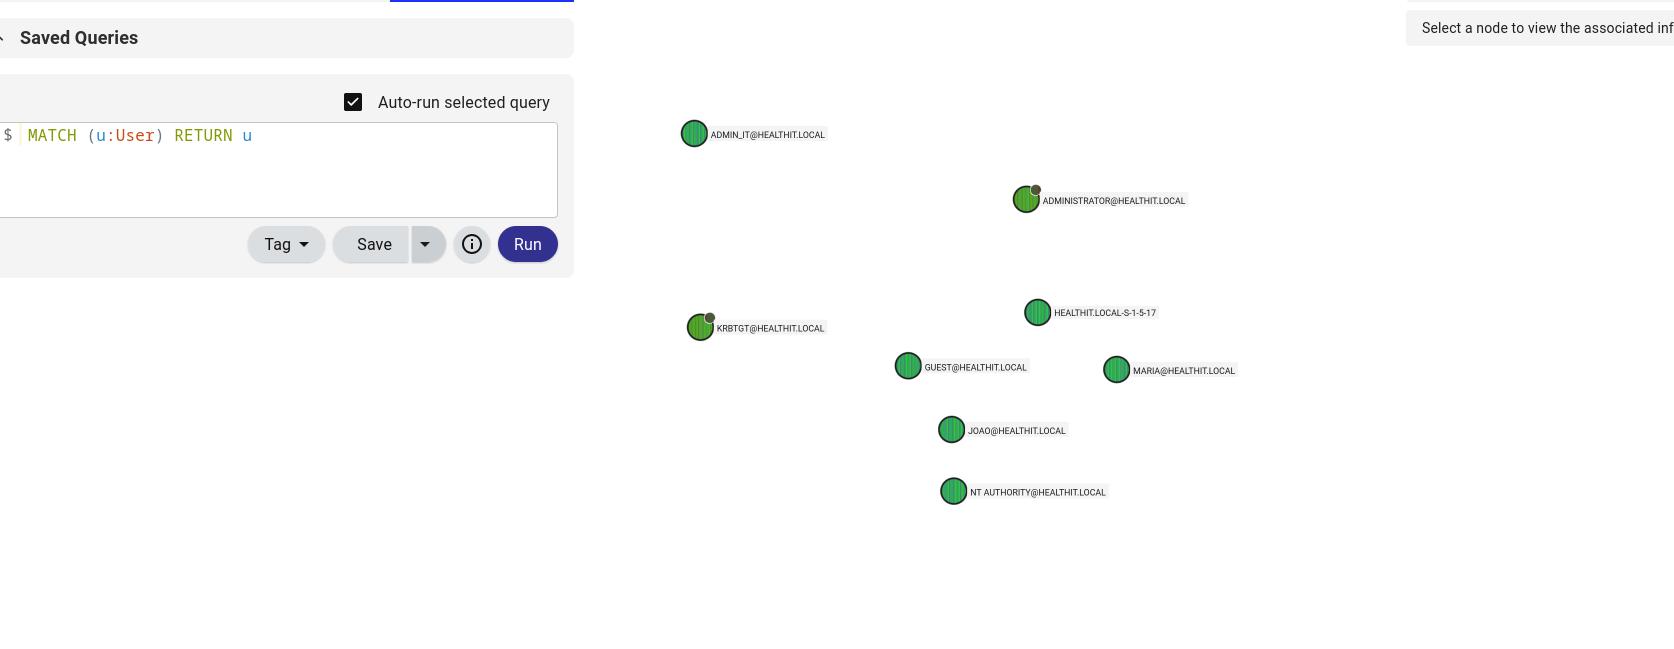
\includegraphics[width=0.8\linewidth]{images/utilizadores_dominio.png}
  \caption{Utilizadores do dominio healthit.local -- Bloodhound}
  \label{fig:bh_users}
\end{figure}

\subsubsection{Grupos do Utilizador JOAO}

O utilizador \texttt{JOAO@HEALTHIT.LOCAL} e membro dos grupos
\textbf{DOMAIN USERS} e \textbf{FINANCE}, o que confirma o acesso
indevido a partilha Finance identificado anteriormente:

\begin{figure}[H]
  \centering
  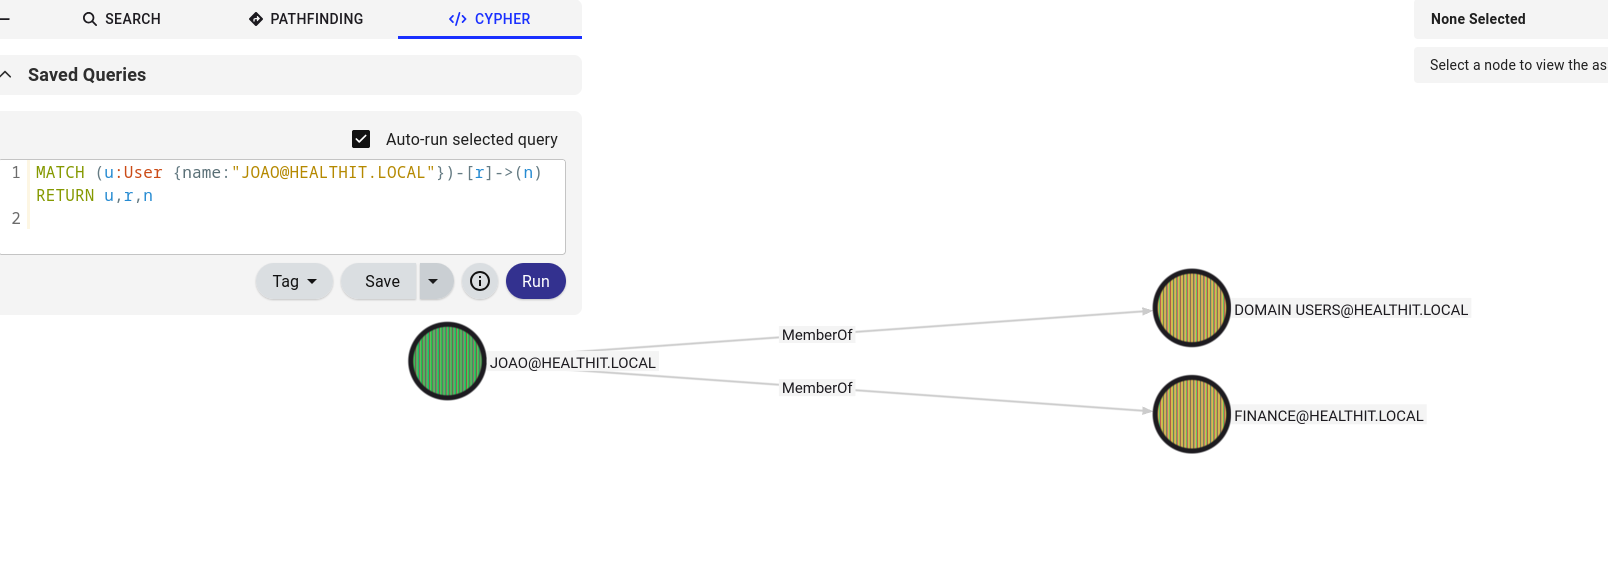
\includegraphics[width=0.8\linewidth]{images/joao_grupos.png}
  \caption{Grupos do utilizador JOAO -- Bloodhound}
  \label{fig:bh_joao_groups}
\end{figure}

\newpage
\subsubsection{Permissoes Excessivas sobre a Conta Administrator}

A analise de caminhos de ataque revelou algo critico: o utilizador
\texttt{JOAO@HEALTHIT.LOCAL} tem permissoes excessivas sobre a
conta \texttt{ADMINISTRATOR@HEALTHIT.LOCAL}:

\begin{figure}[H]
  \centering
  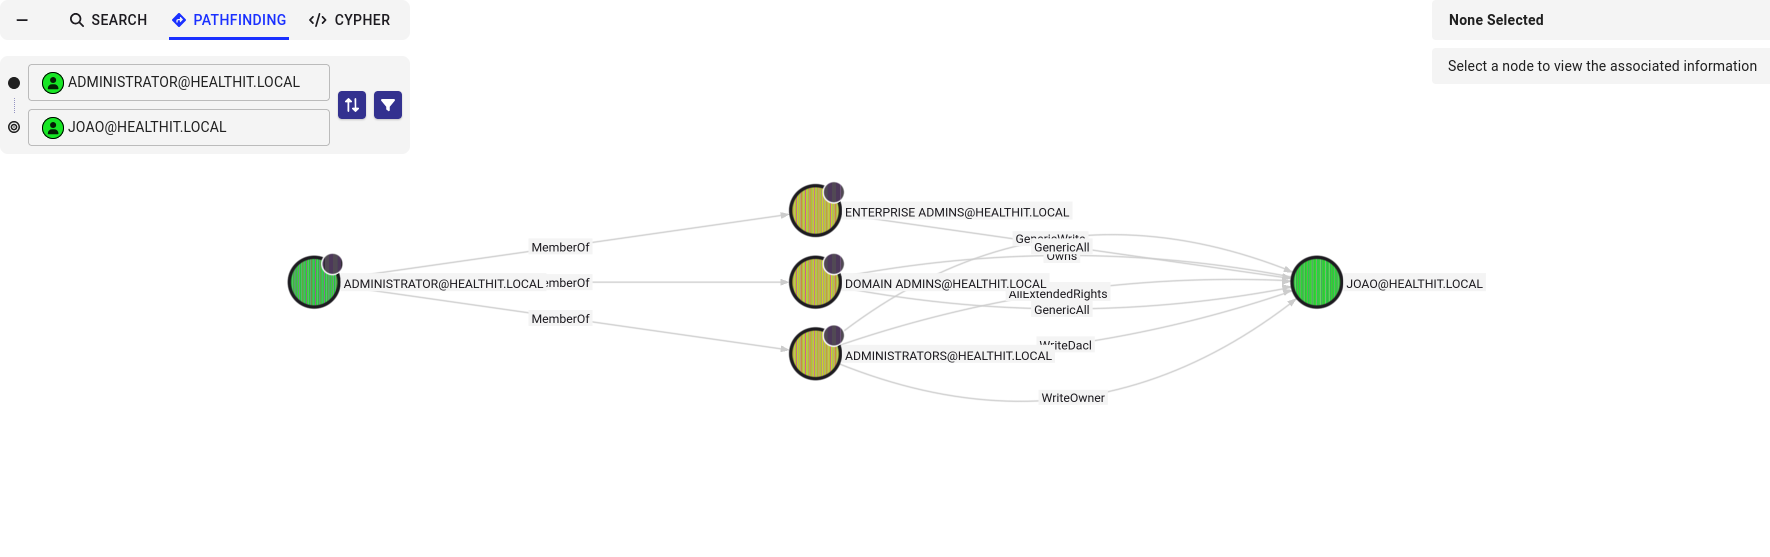
\includegraphics[width=\linewidth]{images/bloodhound_joao_admin.png}
  \caption{Caminho de ataque do JOAO para ADMINISTRATOR -- Bloodhound}
  \label{fig:bh_joao_admin}
\end{figure}

\begin{table}[H]
\centering
\caption{Permissoes do JOAO sobre a conta Administrator}
\begin{tabularx}{\linewidth}{l X}
\toprule
\rowcolor{TableHead}
\thead{Permissao} & \thead{Impacto} \\
\midrule
GenericAll & Controlo total sobre o objeto \\
\rowcolor{TableAlt}
AllExtendedRights & Todos os direitos estendidos, incluindo reset de password \\
Owns & E dono do objeto, podendo alterar qualquer permissao \\
\rowcolor{TableAlt}
WriteDacl & Pode modificar as ACLs do objeto \\
WriteOwner & Pode tomar posse do objeto \\
\bottomrule
\end{tabularx}
\end{table}

\begin{alertbox}
As permissoes identificadas permitem ao utilizador \texttt{joao}, uma
conta comum comprometida via \textit{dark web}, tomar controlo total
sobre a conta \texttt{Administrator} do dominio. Isto resultaria num
\textbf{compromisso total do Active Directory}.
\end{alertbox}


\subsection{Tentativa de Escalada de Privilegios}

Com base nos caminhos de ataque identificados pelo Bloodhound, foram
testadas as seguintes tentativas de escalada de privilegios:

\subsubsection{Reset de Password do Administrator}

Tendo em conta a permissao \textbf{GenericAll}, foi tentado o reset
da password da conta \texttt{Administrator} via RPC:

\begin{lstlisting}[language=bash, caption={Tentativa de reset da password do Administrator}]
net rpc password Administrator newpass123 \
  -U healthit.local/joao%Password1 -S 192.168.50.20
\end{lstlisting}

A tentativa resultou em \texttt{Access is denied}. Apesar das
permissoes identificadas pelo Bloodhound, existem controlos adicionais
que impediam esta acao diretamente via RPC.

\subsubsection{Alteracao de Password da Conta admin\_it}

De seguida, foi testada a conta \texttt{admin\_it}, cujas credenciais
(\texttt{Welcome123}) foram encontradas no ficheiro de passwords. Foi
verificado que qualquer utilizador conseguia alterar a password desta
conta administrativa:

\begin{lstlisting}[language=bash, caption={Alteracao de password da conta admin\_it}]
smbpasswd -r 192.168.50.20 -U admin_it
# Old password: Welcome123
# New password: Welcome1234!
\end{lstlisting}

\begin{figure}[H]
  \centering
  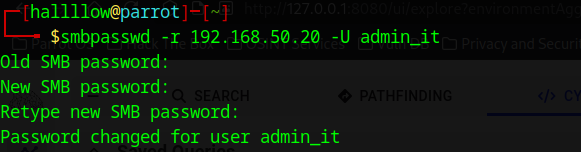
\includegraphics[width=\linewidth]{images/smbpasswd_adminit.png}
  \caption{Alteracao bem sucedida da password da conta admin\_it}
  \label{fig:smbpasswd}
\end{figure}

O sucesso desta operacao confirma uma configuracao incorreta de
privilegios no dominio: um utilizador comum consegue alterar a
password de uma conta administrativa, o que e uma vulnerabilidade
critica de escalada de privilegios.

\subsection{Enumeracao do Dominio -- enum4linux}

Foi feita uma enumeracao completa do dominio com o \texttt{enum4linux}:

\begin{lstlisting}[language=bash, caption={Enumeracao completa do dominio}]
enum4linux -a -u joao -p Password1 192.168.50.20
\end{lstlisting}

\subsubsection{Membros dos Grupos do Dominio}

\begin{figure}[H]
  \centering
  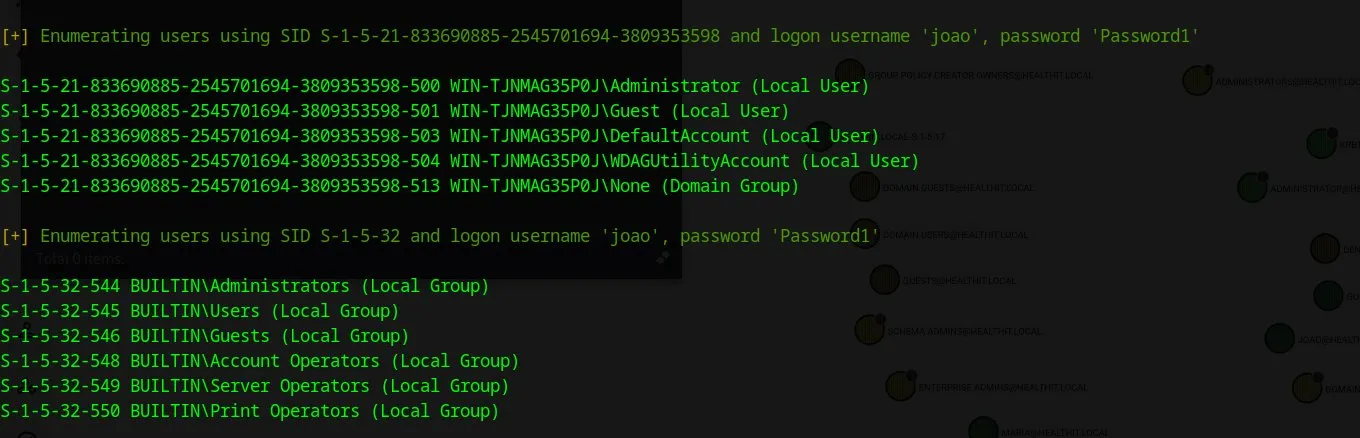
\includegraphics[width=\linewidth]{images/enum4linux_groups.png}
  \caption{Membros dos grupos do dominio HEALTHIT}
  \label{fig:enum4linux_groups}
\end{figure}

A enumeracao revelou informacao relevante sobre a estrutura do
dominio:

\begin{itemize}[itemsep=2pt]
  \item O utilizador \texttt{Administrator} e o unico membro dos
        grupos \textbf{Domain Admins}, \textbf{Enterprise Admins}
        e \textbf{Schema Admins}
  \item O utilizador \texttt{joao} e membro do grupo \textbf{Finance},
        confirmando o acesso indevido a partilha financeira
  \item A conta \texttt{Guest} esta ativa no dominio
  \item Foram identificados dois computadores: \texttt{DESKTOP-30HM9QJ}
        (Windows 10) e \texttt{WIN-TJNMAG35P0J} (Windows Server)
\end{itemize}

\subsubsection{Politica de Passwords do Dominio}

\begin{figure}[H]
  \centering
  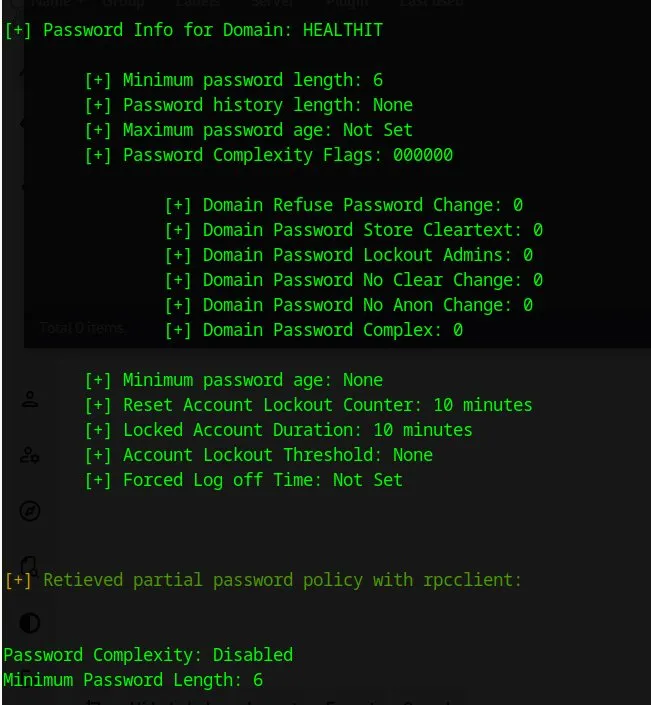
\includegraphics[width=\linewidth]{images/enum4linux_policy.png}
  \caption{Politica de passwords do dominio HEALTHIT}
  \label{fig:enum4linux_policy}
\end{figure}

\begin{table}[H]
\centering
\caption{Analise da Politica de Passwords -- Dominio HEALTHIT}
\begin{tabularx}{\linewidth}{l l X}
\toprule
\rowcolor{TableHead}
\thead{Parametro} & \thead{Valor} & \thead{Problema} \\
\midrule
Comprimento minimo & 6 caracteres & Insuficiente -- minimo recomendado e 12 \\
\rowcolor{TableAlt}
Complexidade & Desativada & Permite passwords simples como \texttt{Password1} \\
Historico & Nenhum & Permite reutilizacao de passwords antigas \\
\rowcolor{TableAlt}
Idade maxima & Nao definida & Passwords nunca expiram \\
Lockout threshold & Nenhum & Permite ataques de forca bruta ilimitados \\
\rowcolor{TableAlt}
Idade minima & Nenhuma & Password pode ser alterada imediatamente \\
\bottomrule
\end{tabularx}
\end{table}

\begin{alertbox}
A ausencia de lockout combinada com a complexidade desativada
permite ataques de forca bruta sem qualquer restricao. Esta
configuracao, aliada as credenciais fracas encontradas na
\textit{dark web} (\texttt{Password1}), representa uma
vulnerabilidade critica de autenticacao.
\end{alertbox}

\subsubsection{Enumeracao de Utilizadores Locais}

\begin{figure}[H]
  \centering
  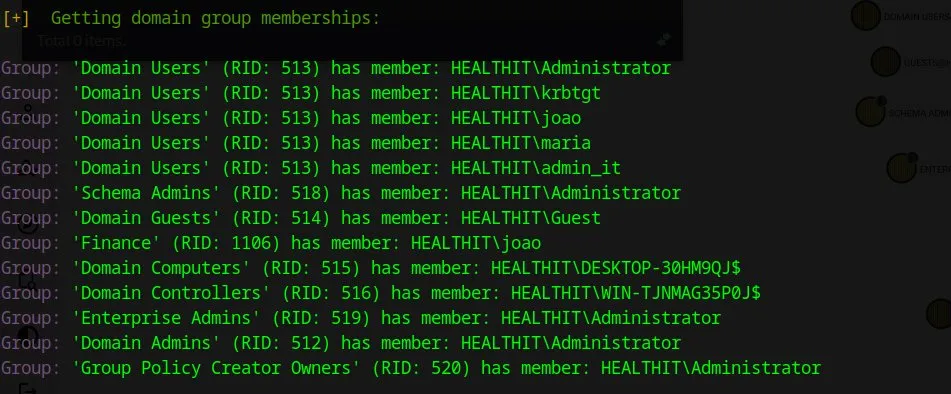
\includegraphics[width=\linewidth]{images/enum4linux_users.png}
  \caption{Utilizadores locais enumerados via SID}
  \label{fig:enum4linux_users}
\end{figure}

A enumeracao via SID revelou contas locais adicionais, confirmando
que a enumeracao de utilizadores e possivel sem privilegios
administrativos -- algo que nao deveria ser possivel numa
infraestrutura bem configurada.

\newpage
\subsection{Analise com Nessus}

Foi realizado um scan com o Nessus Essentials ao Windows Server 2019
para complementar a enumeracao manual. Os resultados do Nessus foram
consistentes com os achados manuais, nao tendo identificado
vulnerabilidades criticas adicionais alem das ja documentadas.
De notar, contudo, que o Nessus confirmou a utilizacao do protocolo
SMBv1 e a exposicao do servico RDP sem controlos de acesso adicionais
(como NLA -- \textit{Network Level Authentication}).

\begin{notebox}
O output completo do scan Nessus encontra-se disponivel nos Anexos
(Secao A.2). A utilizacao do Nessus serviu essencialmente como
validacao cruzada das vulnerabilidades identificadas manualmente.
\end{notebox}

\newpage
\subsection{Resumo de Findings -- Windows Server 2019}

\begin{table}[H]
\centering
\caption{Findings Identificados -- Windows Server 2019}
\begin{tabularx}{\linewidth}{c X c}
\toprule
\rowcolor{TableHead}
\thead{ID} & \thead{Finding} & \thead{Risco} \\
\midrule
WS-01 & Credenciais comprometidas com acesso a partilhas sensiveis & \risk{Critico} \\
\rowcolor{TableAlt}
WS-02 & Ficheiro de passwords em texto claro na partilha Finance & \risk{Critico} \\
WS-03 & Exposicao de PII e dados financeiros na partilha Finance & \risk{Critico} \\
\rowcolor{TableAlt}
WS-04 & Permissoes excessivas do utilizador joao sobre Administrator & \risk{Critico} \\
WS-05 & Politica de passwords fraca, sem complexidade e sem lockout & \risk{Alto} \\
\rowcolor{TableAlt}
WS-06 & Alteracao de password de conta administrativa por utilizador comum & \risk{Alto} \\
WS-07 & SYSVOL e NETLOGON accessiveis por utilizadores comuns & \risk{Medio} \\
\rowcolor{TableAlt}
WS-08 & Conta Guest ativa no dominio & \risk{Medio} \\
WS-09 & Enumeracao de utilizadores possivel sem privilegios & \risk{Medio} \\
\bottomrule
\end{tabularx}
\end{table}

\newpage
% ──────────────────────────────────────────────────────────────
\section{Ubuntu Server 22.04 -- 192.168.50.30}
% ──────────────────────────────────────────────────────────────

\subsection{Enumeracao de Servicos}

\begin{lstlisting}[language=bash, caption={Varrimento de servicos -- Ubuntu Server}]
sudo nmap -Pn -sS -sV -sC 192.168.50.30 -oN scan_ubuntu.txt
\end{lstlisting}

\begin{figure}[H]
  \centering
  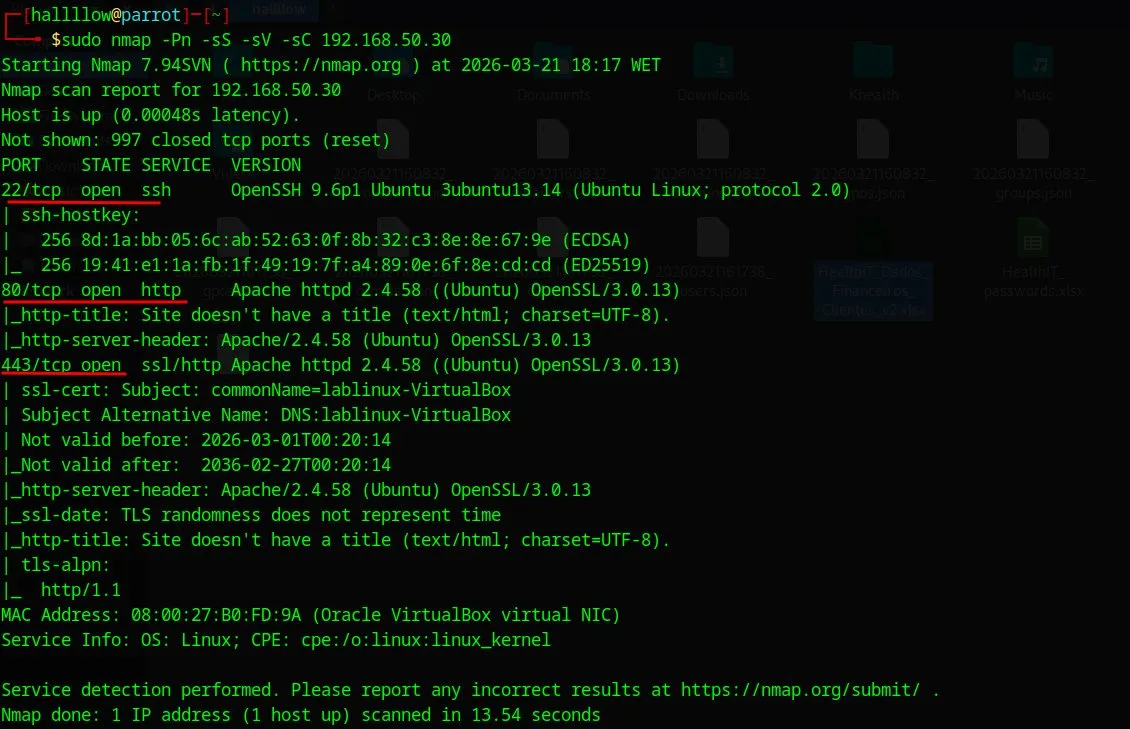
\includegraphics[width=\linewidth]{images/ubuntu_scan.png}
  \caption{Resultado do varrimento Nmap ao Ubuntu Server 22.04}
  \label{fig:scan_ubuntu}
\end{figure}

\begin{table}[H]
\centering
\caption{Portas e Servicos -- 192.168.50.30}
\begin{tabularx}{\linewidth}{c c l X}
\toprule
\rowcolor{TableHead}
\thead{Porta} & \thead{Proto.} & \thead{Servico} & \thead{Observacao} \\
\midrule
22  & TCP & OpenSSH 9.6p1 & SSH exposto sem restricao de acesso \\
\rowcolor{TableAlt}
80  & TCP & Apache 2.4.58 & Aplicacao web em HTTP sem cifra \\
443 & TCP & Apache 2.4.58 & HTTPS com certificado auto-assinado invalido \\
\bottomrule
\end{tabularx}
\end{table}

Da analise do resultado destacam-se os seguintes pontos:

\begin{itemize}[itemsep=2pt]
  \item \textbf{SSH exposto (porta 22)} -- acessivel a partir de
        qualquer host da rede, sem restricao de acesso por IP ou
        utilizacao de chaves publicas como metodo unico
  \item \textbf{Versao do Apache exposta} -- o servidor expoe a
        versao exata (\texttt{2.4.58}) e do OpenSSL (\texttt{3.0.13})
        nos headers HTTP, o que facilita a identificacao de
        vulnerabilidades especificas
  \item \textbf{Certificado SSL auto-assinado} -- o certificado HTTPS
        tem o \textit{Common Name} \texttt{lablinux-VirtualBox},
        nao correspondendo ao dominio real, e nao e emitido por
        uma autoridade certificadora de confianca
  \item \textbf{MySQL nao exposto externamente} -- a porta 3306
        nao esta acessivel, o que e uma boa pratica
\end{itemize}

\subsection{Testes a Aplicacao Web}

A aplicacao web da HealthIT esta acessivel em
\texttt{http://192.168.50.30} e consiste numa plataforma de pesquisa
de pacientes clinicos.

\subsubsection{Exposicao da Query SQL}

Logo na pagina inicial foi identificado algo muito grave: a query
SQL executada no servidor esta visivelmente exposta na interface
para qualquer utilizador, sem necessidade de autenticacao:

\begin{figure}[H]
  \centering
  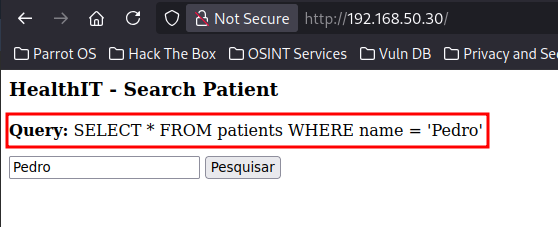
\includegraphics[width=\linewidth]{images/webapp_inicial.png}
  \caption{Aplicacao web -- query SQL exposta na interface}
  \label{fig:webapp_inicial}
\end{figure}

A query \texttt{SELECT * FROM patients WHERE name = '...'} e
apresentada diretamente na pagina, o que revela a estrutura interna
da base de dados e confirma a ausencia de qualquer mecanismo de
sanitizacao de input.

\newpage
\subsubsection{SQL Injection}

Com base na query exposta, foi testada a injeccao SQL diretamente
no campo de pesquisa:

\begin{lstlisting}[caption={Payload de SQL Injection utilizado}]
' OR '1'='1
\end{lstlisting}

\begin{figure}[H]
  \centering
  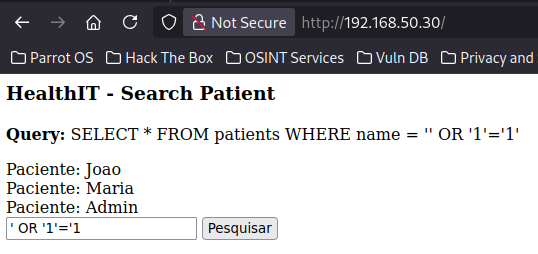
\includegraphics[width=\linewidth]{images/sqli.png}
  \caption{SQL Injection confirmada -- extracao de todos os registos de pacientes}
  \label{fig:sqli}
\end{figure}

O resultado foi imediato: todos os registos de pacientes foram
retornados, confirmando a vulnerabilidade de \textbf{SQL Injection}.

\begin{alertbox}
Esta vulnerabilidade permite a qualquer utilizador sem autenticacao
extrair todos os dados clinicos armazenados, incluindo nomes, dados
pessoais e registos medicos de pacientes. Tratando-se de dados de
saude, a exploracao desta falha constitui uma violacao grave do RGPD
(Artigo 9.o -- categorias especiais de dados e Artigo 32.o --
seguranca do tratamento), podendo resultar em multas ate
\textbf{4\% do volume de negocios anual} da empresa.
\end{alertbox}

\subsubsection{Extracao de Dados via SQLMap}

Para confirmar o impacto real da vulnerabilidade, foi utilizado
o \texttt{sqlmap} para extracao automatizada dos dados:

\begin{lstlisting}[language=bash, caption={Identificacao das bases de dados}]
sqlmap -u "http://192.168.50.30/" --data="name=test" --dbs --batch
\end{lstlisting}

\begin{figure}[H]
  \centering
  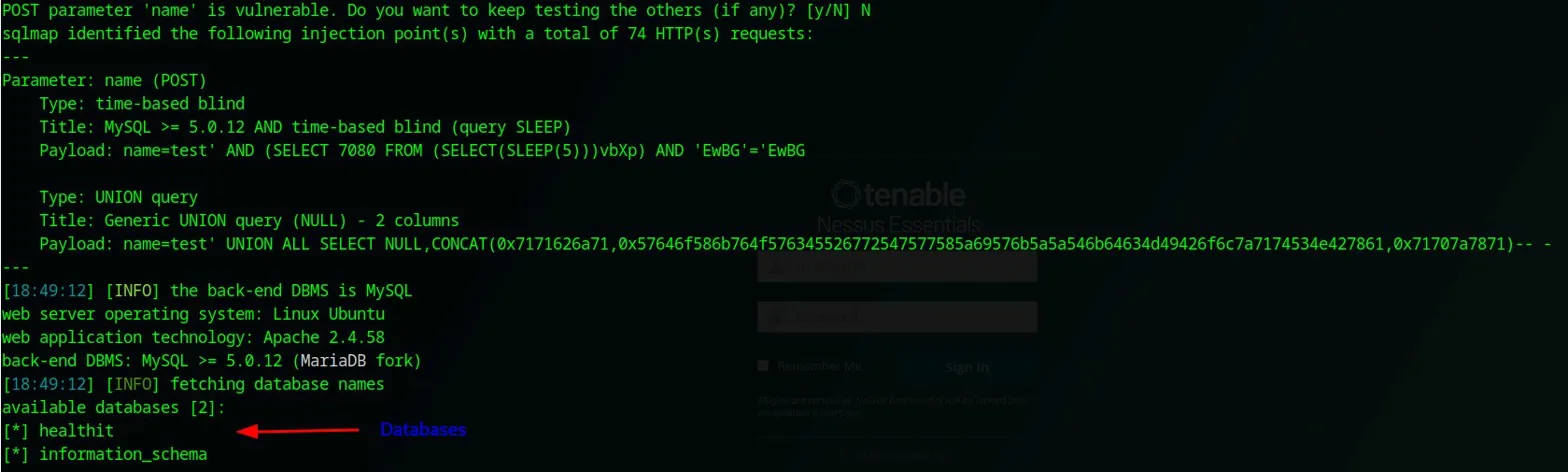
\includegraphics[width=\linewidth]{images/sqlmap_dbs.png}
  \caption{SQLMap -- identificacao do tipo de injeccao e bases de dados}
  \label{fig:sqlmap_dbs}
\end{figure}

O sqlmap confirmou dois tipos de SQL Injection:
\begin{itemize}[itemsep=2pt]
  \item \textbf{Time-Based Blind} -- injeccao baseada em tempo de resposta
  \item \textbf{UNION Query} -- injeccao por uniao de queries
\end{itemize}

Foram identificadas duas bases de dados: \texttt{healthit} e
\texttt{information\_schema}.

\begin{lstlisting}[language=bash, caption={Extracao de tabelas da base de dados healthit}]
sqlmap -u "http://192.168.50.30/" --data="name=test" \
  -D healthit --tables --batch
\end{lstlisting}

\begin{figure}[H]
  \centering
  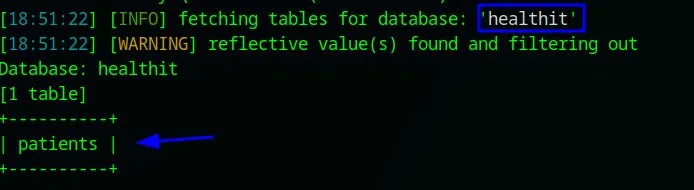
\includegraphics[width=\linewidth]{images/sqlmap_tables.png}
  \caption{SQLMap -- tabela patients identificada na base de dados healthit}
  \label{fig:sqlmap_tables}
\end{figure}

\begin{lstlisting}[language=bash, caption={Extracao de registos da tabela patients}]
sqlmap -u "http://192.168.50.30/" --data="name=test" \
  -D healthit -T patients --dump --batch
\end{lstlisting}

\begin{figure}[H]
  \centering
  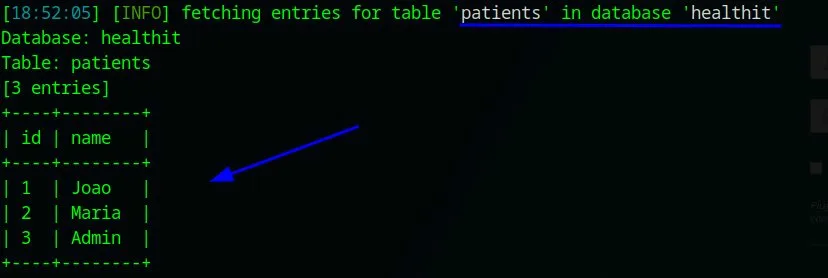
\includegraphics[width=\linewidth]{images/sqlmap_dump.png}
  \caption{SQLMap -- registos extraidos da tabela patients}
  \label{fig:sqlmap_dump}
\end{figure}

\begin{alertbox}
A exploracao da vulnerabilidade de SQL Injection permitiu extrair
todos os registos de pacientes sem qualquer autenticacao. Num cenario
real, um atacante poderia extrair, modificar ou eliminar todos os
dados clinicos armazenados na empresa.
\end{alertbox}

\newpage
\subsubsection{Analise do Certificado SSL}

\begin{lstlisting}[language=bash, caption={Analise do certificado SSL}]
curl -vk https://192.168.50.30 2>&1 | grep -A 10 "SSL"
\end{lstlisting}

\begin{figure}[H]
  \centering
  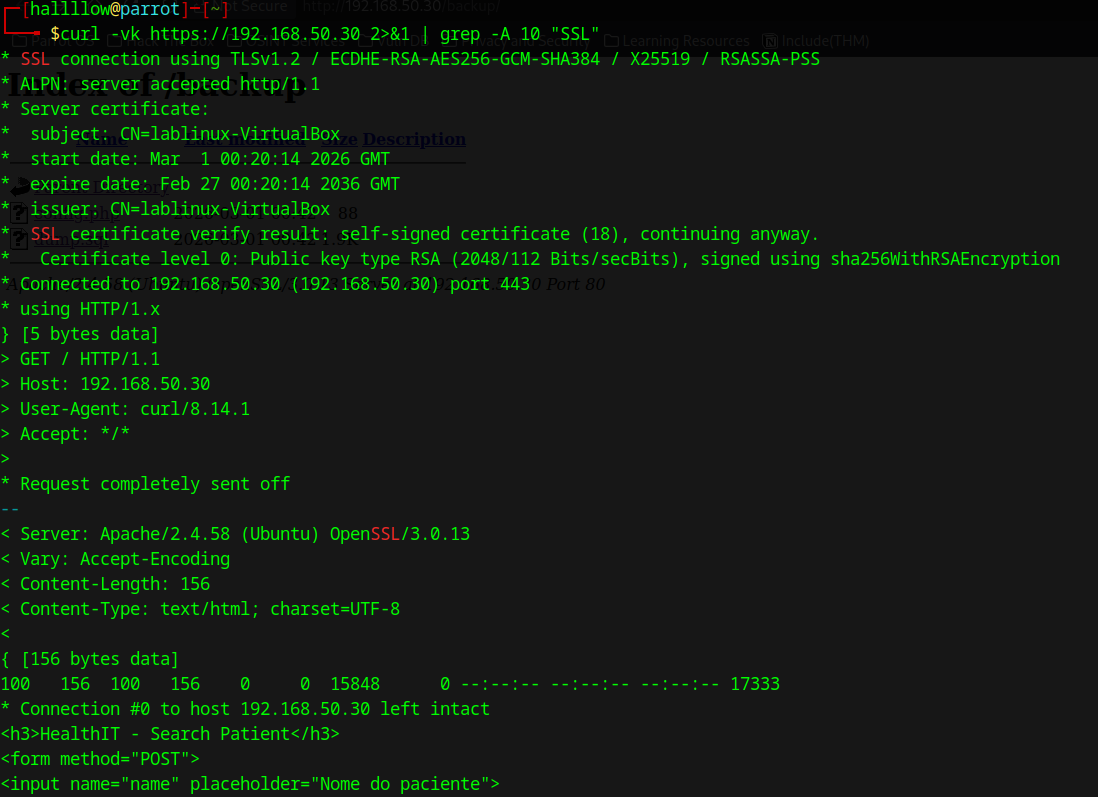
\includegraphics[width=\linewidth]{images/ssl_cert.png}
  \caption{Certificado SSL auto-assinado -- Ubuntu Server}
  \label{fig:ssl_cert}
\end{figure}

A analise revelou tres falhas no certificado SSL:

\begin{itemize}[itemsep=2pt]
  \item \textbf{Certificado auto-assinado} -- nao emitido por
        autoridade certificadora de confianca
  \item \textbf{Common Name incorreto} -- \texttt{lablinux-VirtualBox}
        nao corresponde ao dominio da aplicacao
  \item \textbf{Versao do servidor exposta} -- header
        \texttt{Apache/2.4.58 (Ubuntu) OpenSSL/3.0.13} visivel
        nas respostas HTTP
\end{itemize}

\newpage
\subsubsection{Scan com Nuclei}

\begin{lstlisting}[language=bash, caption={Scan Nuclei ao Ubuntu Server}]
nuclei -u http://192.168.50.30 -o nuclei_ubuntu.txt
\end{lstlisting}

\begin{figure}[H]
  \centering
  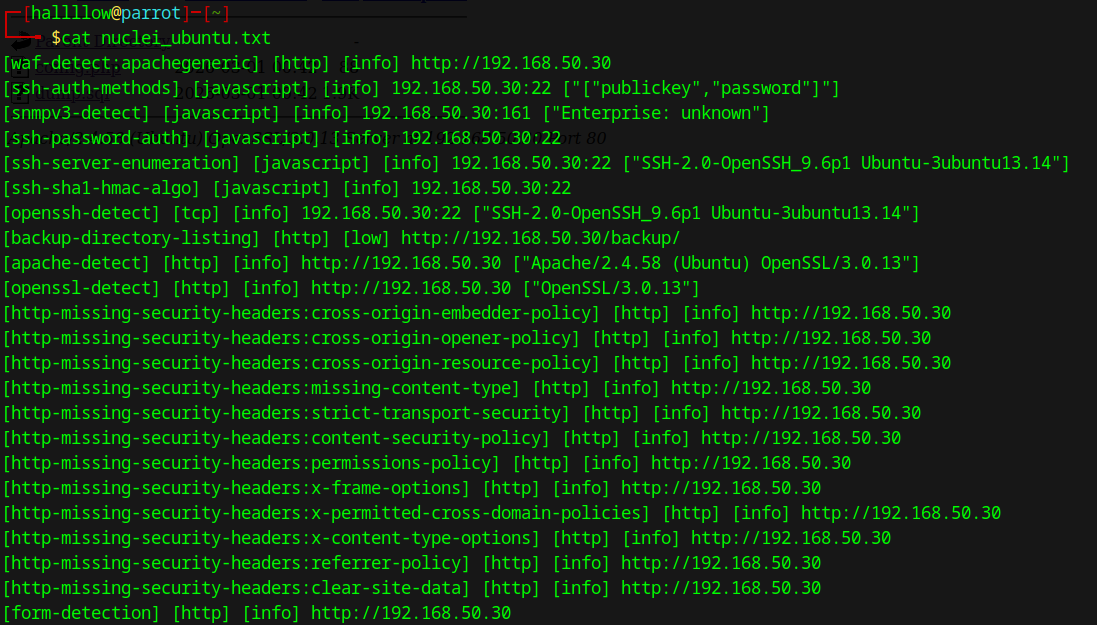
\includegraphics[width=\linewidth]{images/nuclei_ubuntu.png}
  \caption{Resultado do scan Nuclei ao Ubuntu Server}
  \label{fig:nuclei_ubuntu}
\end{figure}

\begin{table}[H]
\centering
\caption{Findings Nuclei -- Ubuntu Server 192.168.50.30}
\begin{tabularx}{\linewidth}{l l X}
\toprule
\rowcolor{TableHead}
\thead{Finding} & \thead{Severidade} & \thead{Observacao} \\
\midrule
Diretorio /backup exposto & Low & Backup da BD accessivel sem autenticacao \\
\rowcolor{TableAlt}
SSH permite password auth & Info & Autenticacao SSH por password ativa \\
SSH SHA1 HMAC & Info & Algoritmo de hash fraco no SSH \\
\rowcolor{TableAlt}
SNMP exposto (porta 161) & Info & Servico SNMP accessivel na rede \\
Headers de seguranca em falta & Info & CSP, HSTS, X-Frame-Options ausentes \\
\rowcolor{TableAlt}
Versao Apache exposta & Info & Apache/2.4.58 visivel nos headers \\
\bottomrule
\end{tabularx}
\end{table}

De notar que o diretorio \texttt{/backup} esta acessivel sem
autenticacao, o que pode expor ficheiros de backup da base de dados
diretamente na web. Este finding sera incluido na avaliacao de risco
como VUL associada ao Ubuntu Server.

\subsubsection{Cross-Site Scripting (XSS)}

Durante os testes a aplicacao web foi identificado um XSS Refletido
no campo de pesquisa de pacientes. O payload injetado foi executado
pelo browser sem qualquer sanitizacao:

\begin{lstlisting}[caption={Payload XSS utilizado}]
<script>alert(1)</script>
\end{lstlisting}

\begin{figure}[H]
  \centering
  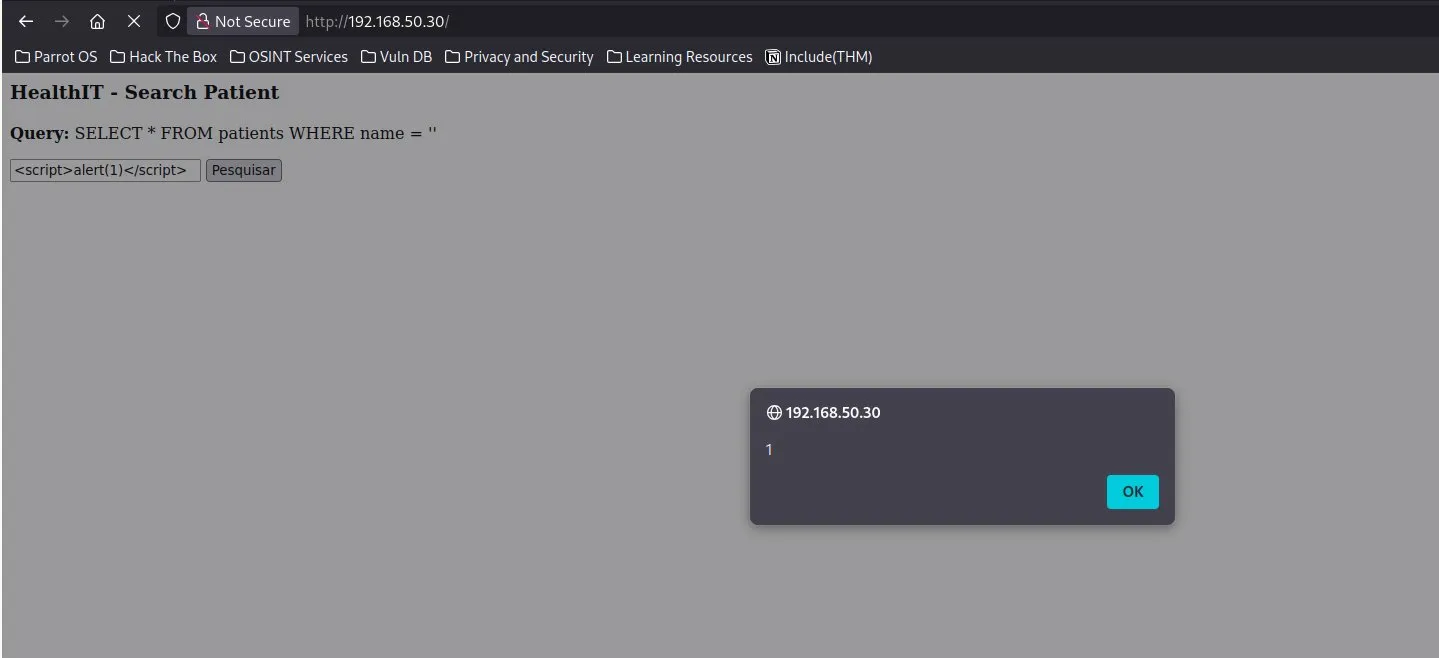
\includegraphics[width=\linewidth]{images/xss.png}
  \caption{XSS Refletido confirmado na aplicacao clinica HealthIT}
  \label{fig:xss}
\end{figure}

Esta vulnerabilidade pode ser usada para:

\begin{itemize}[itemsep=2pt]
  \item \textbf{Roubo de sessao} -- captura de cookies de sessao
        de utilizadores autenticados
  \item \textbf{Phishing} -- redirecionamento para paginas falsas
  \item \textbf{Keylogging} -- captura de dados introduzidos
        na aplicacao clinica
  \item \textbf{Defacement} -- alteracao da interface da aplicacao
\end{itemize}

\begin{alertbox}
Numa aplicacao clinica que processa dados de saude, o roubo de
sessao via XSS poderia permitir a um atacante aceder aos registos
clinicos de pacientes em nome de um utilizador legitimo,
constituindo uma violacao do RGPD (Artigo 32.o).
\end{alertbox}

\newpage
\subsection{Resumo de Findings -- Ubuntu Server 22.04}

\begin{table}[H]
\centering
\caption{Findings Identificados -- Ubuntu Server 22.04}
\begin{tabularx}{\linewidth}{c X c}
\toprule
\rowcolor{TableHead}
\thead{ID} & \thead{Finding} & \thead{Risco} \\
\midrule
UB-01 & SQL Injection na aplicacao web clinica & \risk{Critico} \\
\rowcolor{TableAlt}
UB-02 & Cross-Site Scripting (XSS) Refletido & \risk{Alto} \\
UB-03 & Query SQL exposta na interface da aplicacao & \risk{Alto} \\
\rowcolor{TableAlt}
UB-04 & Diretorio /backup accessivel sem autenticacao & \risk{Alto} \\
UB-05 & Certificado SSL auto-assinado com CN incorreto & \risk{Medio} \\
\rowcolor{TableAlt}
UB-06 & Headers de seguranca HTTP em falta & \risk{Medio} \\
UB-07 & SNMP exposto na porta 161 & \risk{Medio} \\
\rowcolor{TableAlt}
UB-08 & Versao do Apache e OpenSSL expostas & \risk{Baixo} \\
UB-09 & SSH permite autenticacao por password & \risk{Baixo} \\
\bottomrule
\end{tabularx}
\end{table}

\begin{notebox}
O utilizador MySQL (\texttt{app@localhost}) opera com privilegios
minimos (\texttt{USAGE}), o que e uma boa pratica de seguranca e
impediu a escalada do ataque para execucao remota de codigo via
SQL Injection. No entanto, a vulnerabilidade de SQL Injection
continua a ser critica dado o acesso aos dados clinicos.
\end{notebox}

\newpage
% ──────────────────────────────────────────────────────────────
\section{Windows 10 -- 192.168.50.40}
% ──────────────────────────────────────────────────────────────

\subsection{Enumeracao de Servicos}

\begin{lstlisting}[language=bash, caption={Varrimento de servicos -- Windows 10}]
sudo nmap -Pn -sS -sV -sC 192.168.50.40
\end{lstlisting}

\begin{figure}[H]
  \centering
  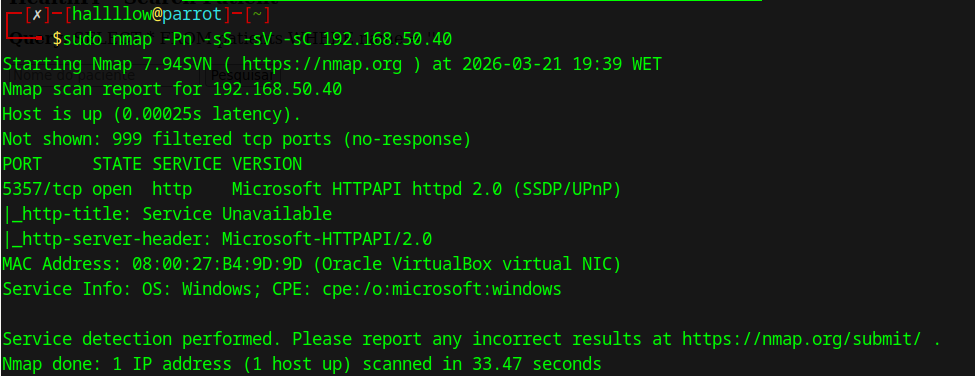
\includegraphics[width=\linewidth]{images/win10_scan.png}
  \caption{Resultado do varrimento Nmap ao Windows 10}
  \label{fig:scan_win10}
\end{figure}

\begin{table}[H]
\centering
\caption{Portas e Servicos -- 192.168.50.40}
\begin{tabularx}{\linewidth}{c c l X}
\toprule
\rowcolor{TableHead}
\thead{Porta} & \thead{Proto.} & \thead{Servico} & \thead{Observacao} \\
\midrule
5357 & TCP & Microsoft HTTPAPI & SSDP/UPnP -- descoberta de rede \\
\bottomrule
\end{tabularx}
\end{table}

O Windows 10 apresenta uma superficie de ataque reduzida com o
firewall ativo. O servico \textbf{UPnP} exposto na porta 5357 pode
ser usado para ataques de descoberta e enumeracao de rede, mas nao
representa um risco critico por si so.

\subsection{Acesso com Credenciais Comprometidas -- admin\_it}

\subsubsection{Enumeracao de Utilizadores Locais}

Com acesso fisico ao Windows 10 atraves da conta \texttt{maria},
foi feita a enumeracao dos utilizadores locais:

\begin{lstlisting}[caption={Enumeracao de utilizadores locais}]
net user
\end{lstlisting}

\begin{table}[H]
\centering
\caption{Utilizadores Locais -- Windows 10}
\begin{tabularx}{\linewidth}{l l X}
\toprule
\rowcolor{TableHead}
\thead{Utilizador} & \thead{Ativo} & \thead{Observacao} \\
\midrule
Administrator  & Sim & Conta de administrador local \\
\rowcolor{TableAlt}
Default Account & Sim & Conta padrao Windows \\
defaultuser0   & Sim & Conta de configuracao inicial \\
\rowcolor{TableAlt}
Guest          & Sim & Conta de convidado ativa \\
Labtest        & Sim & Conta de teste com privilegios de administrador \\
\rowcolor{TableAlt}
maria          & Sim & Utilizadora com credenciais comprometidas \\
\bottomrule
\end{tabularx}
\end{table}

\subsubsection{Conta Labtest sem Password Obrigatoria}

A analise da conta \texttt{Labtest} revelou que esta pertence ao
grupo \textbf{Administrators} e nao tem password obrigatoria:

\begin{figure}[H]
  \centering
  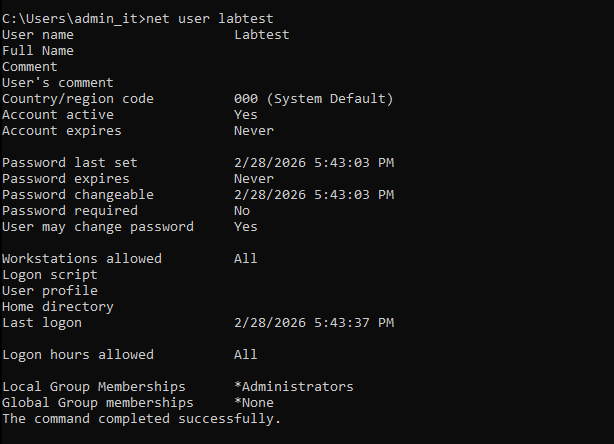
\includegraphics[width=\linewidth]{images/labtest_user.png}
  \caption{Conta Labtest -- administrador local sem password obrigatoria}
  \label{fig:labtest}
\end{figure}

\begin{alertbox}
A conta \texttt{Labtest} e membro do grupo \textbf{Administrators}
e esta configurada com \texttt{Password required: No}. Apesar de nao
ter sido possivel autenticar sem password neste teste, esta
configuracao representa uma vulnerabilidade critica de gestao de
contas privilegiadas que deve ser corrigida imediatamente.
\end{alertbox}

\newpage
\subsubsection{Reutilizacao de Credenciais -- Movimento Lateral}

As credenciais da conta \texttt{admin\_it} encontradas na partilha
Finance foram testadas no Windows 10, confirmando a reutilizacao
de credenciais entre sistemas do dominio:

\begin{figure}[H]
  \centering
  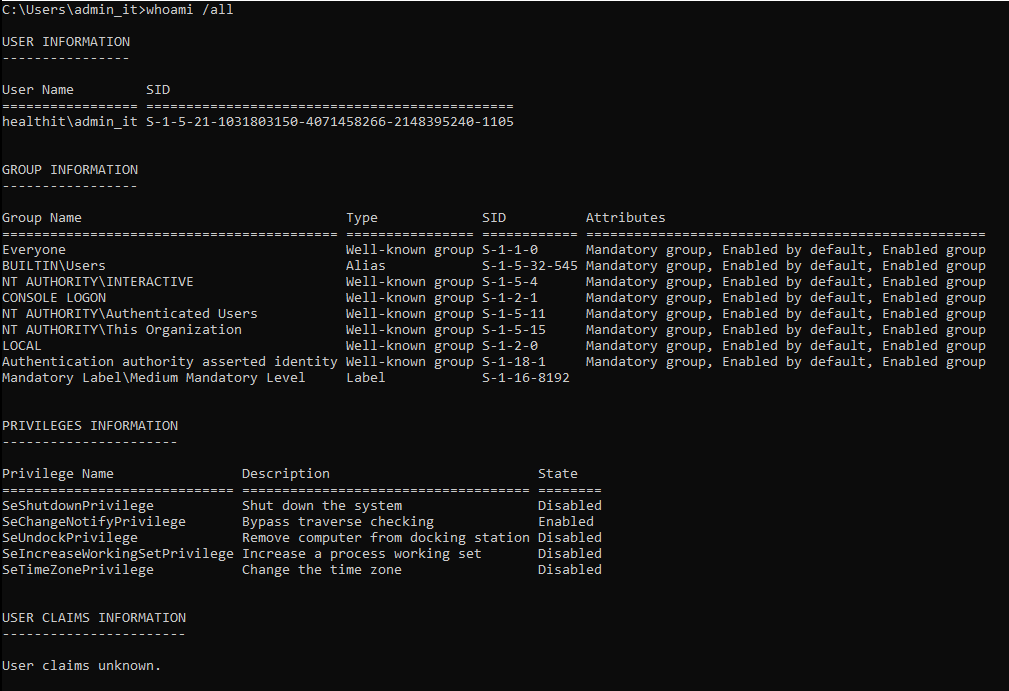
\includegraphics[width=\linewidth]{images/whoami_adminit.png}
  \caption{Acesso ao Windows 10 com credenciais comprometidas -- admin\_it}
  \label{fig:whoami_adminit}
\end{figure}

O resultado do \texttt{whoami /all} confirma o acesso autenticado
como \texttt{healthit\textbackslash admin\_it} no Windows 10,
demonstrando movimento lateral bem sucedido. Este acesso foi possivel
gracas a reutilizacao das credenciais encontradas na partilha Finance.

\subsection{Resumo de Findings -- Windows 10}

\begin{table}[H]
\centering
\caption{Findings Identificados -- Windows 10}
\begin{tabularx}{\linewidth}{c X c}
\toprule
\rowcolor{TableHead}
\thead{ID} & \thead{Finding} & \thead{Risco} \\
\midrule
W10-01 & Conta Labtest com privilegios de administrador sem password obrigatoria & \risk{Critico} \\
\rowcolor{TableAlt}
W10-02 & Reutilizacao de credenciais -- admin\_it acede ao Windows 10 & \risk{Alto} \\
W10-03 & Conta Guest ativa no sistema & \risk{Medio} \\
\rowcolor{TableAlt}
W10-04 & UPnP exposto na porta 5357 & \risk{Baixo} \\
\bottomrule
\end{tabularx}
\end{table}

O Windows 10 apresenta o firewall ativo como ponto positivo, limitando
a superficie de ataque remoto. No entanto, a conta \texttt{Labtest}
sem password obrigatoria e a reutilizacao de credenciais do dominio
representam riscos criticos em caso de acesso fisico ou movimento
lateral.

\newpage
% ──────────────────────────────────────────────────────────────
\section{Analise de Trafego -- Wireshark}
% ──────────────────────────────────────────────────────────────

Durante a execucao dos testes foi capturado trafego da rede interna
com o Wireshark, revelando comunicacoes sem cifra com exposicao de
dados sensiveis.

\subsection{Trafego HTTP em Claro}

\begin{figure}[H]
  \centering
  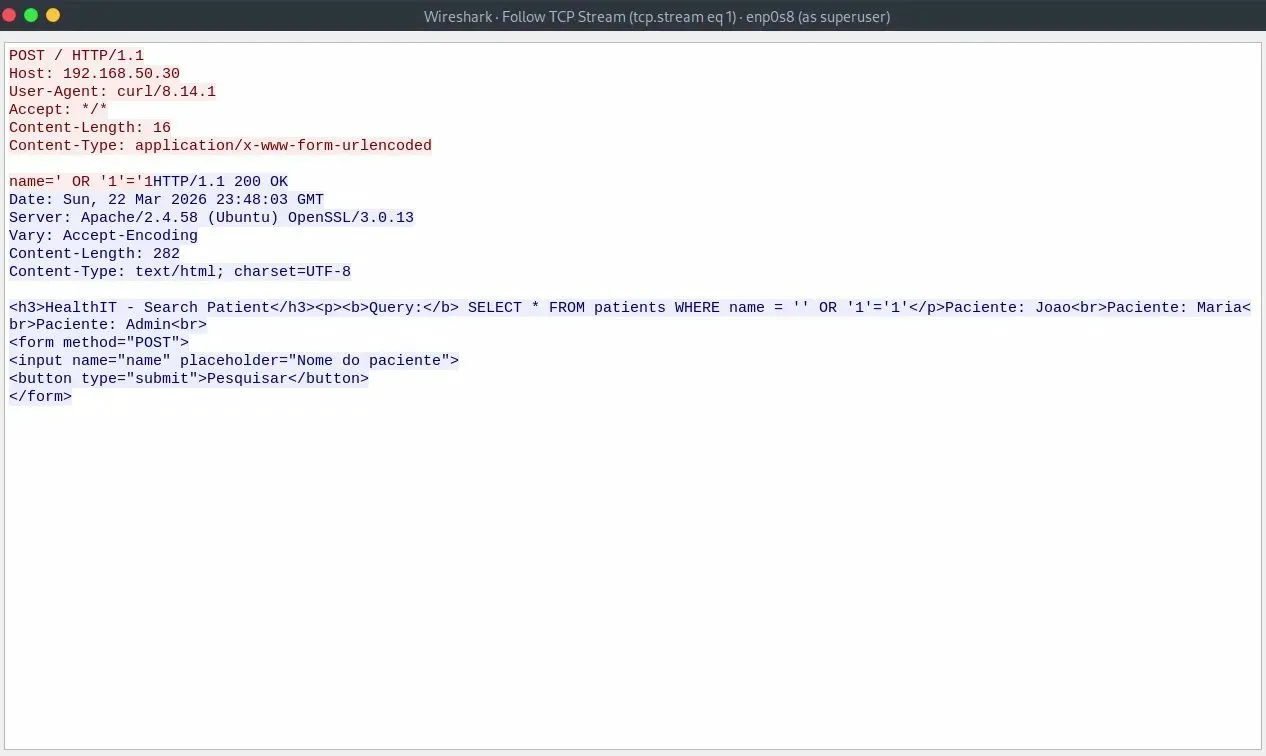
\includegraphics[width=\linewidth]{images/wireshark_http.png}
  \caption{Trafego HTTP capturado -- dados de pacientes em claro}
  \label{fig:wireshark_http}
\end{figure}

A analise do trafego HTTP confirmou que a aplicacao web transmite
dados sem qualquer cifra, expondo:

\begin{itemize}[itemsep=2pt]
  \item \textbf{Payloads de SQL Injection} visiveis em claro
        (\texttt{name=' OR '1'='1})
  \item \textbf{Query SQL} exposta na resposta do servidor
  \item \textbf{Dados de pacientes} transmitidos sem cifra
        (Joao, Maria, Admin)
  \item \textbf{Versao do servidor} exposta nos headers
\end{itemize}

\subsection{Trafego SMB -- Autenticacao NTLM}

\begin{figure}[H]
  \centering
  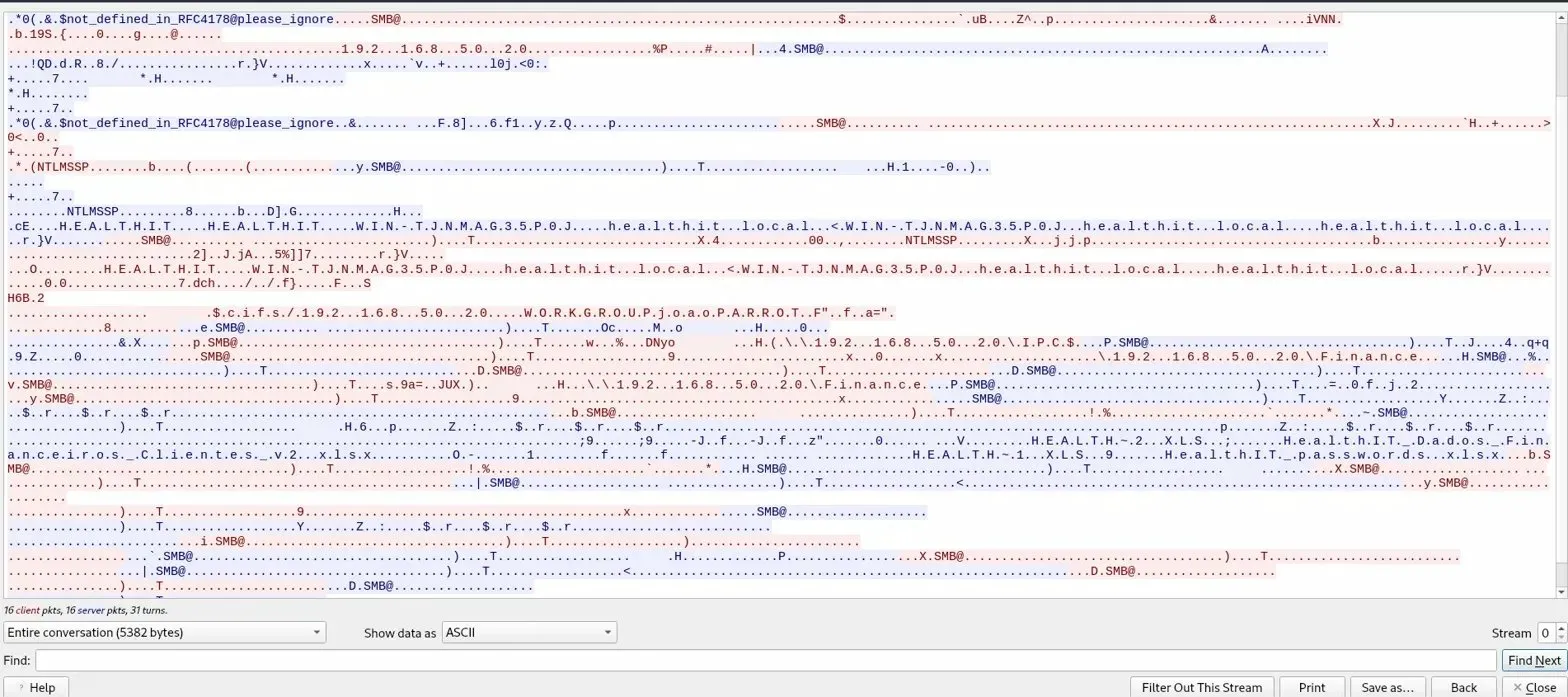
\includegraphics[width=\linewidth]{images/wireshark_smb.png}
  \caption{Trafego SMB capturado -- autenticacao NTLM e ficheiros expostos}
  \label{fig:wireshark_smb}
\end{figure}

A analise do trafego SMB revelou:

\begin{itemize}[itemsep=2pt]
  \item \textbf{Autenticacao NTLM} visivel em claro, com hashes
        capturaveis para ataques de Pass-the-Hash
  \item \textbf{Nomes de ficheiros sensiveis} expostos no trafego:
        \texttt{HealthIT\_Dados\_Financeiros\_Clientes\_v2.xlsx}
        e \texttt{HealthIT\_passwords.xlsx}
  \item \textbf{Estrutura da rede} exposta, com dominio
        \texttt{HEALTHIT} e servidor \texttt{WIN-TJNMAG35P0J}
        visiveis
\end{itemize}

\begin{alertbox}
A ausencia de cifra no trafego HTTP e a utilizacao de NTLM no SMB
permitem a qualquer atacante com acesso a rede interna capturar dados
clinicos de pacientes e hashes de autenticacao, facilitando ataques
de movimento lateral sem necessidade de conhecer as passwords em
texto claro.
\end{alertbox}


% ══════════════════════════════════════════════════════════════
\chapter{Avaliacao de Risco}
% ══════════════════════════════════════════════════════════════

\section{Metodologia de Classificacao}

Cada vulnerabilidade foi classificada segundo duas dimensoes:
\textbf{Probabilidade de Exploracao} e \textbf{Impacto no Negocio},
numa escala de tres niveis (Baixo, Medio, Alto). O cruzamento das
duas dimensoes determina o \textbf{Nivel de Risco Final}. A avaliacao
de impacto teve em conta o tipo e volume de dados envolvidos, o
impacto legal (RGPD), o impacto financeiro, o impacto reputacional
e a possibilidade de propagacao lateral.

\section{Matriz de Probabilidade x Impacto}

\begin{table}[H]
\centering
\caption{Matriz de Risco}
\begin{tabular}{l c c c}
\toprule
\rowcolor{TableHead}
\thead{Impacto $\downarrow$ / Probabilidade $\rightarrow$}
  & \thead{Baixa} & \thead{Media} & \thead{Alta} \\
\midrule
\textbf{Alto}
  & \cellcolor{Medium!60}Medio
  & \cellcolor{High!70}\color{white}Alto
  & \cellcolor{Critical}\color{white}\bfseries Critico \\
\midrule
\textbf{Medio}
  & \cellcolor{Low!60}\color{white}Baixo
  & \cellcolor{Medium!60}Medio
  & \cellcolor{High!70}\color{white}Alto \\
\midrule
\textbf{Baixo}
  & \cellcolor{Low!60}\color{white}Baixo
  & \cellcolor{Low!60}\color{white}Baixo
  & \cellcolor{Medium!60}Medio \\
\bottomrule
\end{tabular}
\end{table}

\section{Findings}

% ── VUL-01 ────────────────────────────────────────────────────
\begin{finding}{VUL-01 -- Credenciais Comprometidas na Dark Web}

\begin{tabular}{@{}ll@{}}
  \small\color{TextGray}Ativo afetado   & \texttt{192.168.50.20} -- Windows Server 2019 \\[3pt]
  \small\color{TextGray}Nivel de risco  & \risk{Critico} \\[3pt]
  \small\color{TextGray}Probabilidade   & Alta \\[3pt]
  \small\color{TextGray}Impacto negocio & Alto \\
\end{tabular}

\vspace{8pt}
\textbf{Descricao tecnica}

As credenciais do utilizador \texttt{joao} (\texttt{Password1}) foram
encontradas na \textit{dark web} e notificadas pelo CNCS. A password
nao cumpre qualquer requisito de complexidade e nunca foi alterada.
Com estas credenciais foi possivel autenticar em multiplos servicos
da infraestrutura, incluindo SMB e potencialmente RDP.

\vspace{6pt}
\textbf{Evidencia}

Autenticacao bem sucedida via SMB com as credenciais comprometidas,
com acesso a partilhas sensiveis incluindo \texttt{Finance},
\texttt{SYSVOL} e \texttt{NETLOGON} (Figura~\ref{fig:smbclient_enum}).

\vspace{4pt}
\textbf{Impacto organizacional}
\begin{itemize}[itemsep=1pt]
  \item \textbf{Tipo de dados:} Credenciais de dominio, informacao financeira, PII
  \item \textbf{Impacto RGPD (Art. 32.o):} Acesso nao autorizado a dados pessoais
  \item \textbf{Impacto financeiro:} Acesso direto a dados financeiros de clientes
  \item \textbf{Impacto reputacional:} Elevado -- credenciais expostas publicamente
  \item \textbf{Propagacao lateral:} Alta -- credenciais validas em multiplos sistemas
\end{itemize}

\vspace{4pt}
\textbf{Recomendacao}

Revogar imediatamente as credenciais comprometidas e forccar o reset
de password de todos os utilizadores do dominio. Implementar
autenticacao multifator (MFA). Ativar monitorizacao continua de
credenciais comprometidas (ex: integracoes com Have I Been Pwned
ou alertas do CNCS).
\end{finding}

\vspace{0.8em}

\newpage
% ── VUL-02 ────────────────────────────────────────────────────
\begin{finding}{VUL-02 -- Ficheiro de Passwords em Texto Claro}

\begin{tabular}{@{}ll@{}}
  \small\color{TextGray}Ativo afetado   & \texttt{192.168.50.20} -- Partilha Finance \\[3pt]
  \small\color{TextGray}Nivel de risco  & \risk{Critico} \\[3pt]
  \small\color{TextGray}Probabilidade   & Alta \\[3pt]
  \small\color{TextGray}Impacto negocio & Alto \\
\end{tabular}

\vspace{8pt}
\textbf{Descricao tecnica}

O ficheiro \texttt{HealthIT\_passwords.xlsx} estava armazenado na
partilha \texttt{Finance}, acessivel a qualquer utilizador do dominio
com as credenciais comprometidas. O ficheiro continha credenciais em
texto claro de multiplos sistemas, incluindo credenciais root do
servidor Ubuntu e credenciais de administracao da base de dados.
Nao existe qualquer justificacao tecnica para armazenar passwords
desta forma.

\vspace{6pt}
\textbf{Evidencia}

Download e analise do ficheiro via \texttt{smbclient}, revelando
credenciais de 6 sistemas distintos em texto claro
(Figura~\ref{fig:passwords_xlsx}).

\vspace{4pt}
\textbf{Impacto organizacional}
\begin{itemize}[itemsep=1pt]
  \item \textbf{Tipo de dados:} Credenciais de multiplos sistemas criticos
  \item \textbf{Impacto RGPD (Art. 32.o):} Compromisso de sistemas com dados pessoais
  \item \textbf{Impacto financeiro:} Acesso a todos os sistemas da infraestrutura
  \item \textbf{Impacto reputacional:} Severo -- gestao negligente de credenciais
  \item \textbf{Propagacao lateral:} Critica -- credenciais de root e BD expostas
\end{itemize}

\vspace{4pt}
\textbf{Recomendacao}

Eliminar imediatamente o ficheiro da partilha Finance. Revogar e
alterar todas as credenciais expostas. Implementar um gestor de
passwords empresarial (ex: Bitwarden Teams, CyberArk). Nunca
armazenar credenciais em ficheiros de texto ou folhas de calculo.
Restringir o acesso a partilha Finance apenas ao grupo de utilizadores
com necessidade efetiva.
\end{finding}

\vspace{0.8em}

% ── VUL-03 ────────────────────────────────────────────────────
\begin{finding}{VUL-03 -- SQL Injection na Aplicacao Web Clinica}

\begin{tabular}{@{}ll@{}}
  \small\color{TextGray}Ativo afetado   & \texttt{192.168.50.30} -- Ubuntu Server 22.04 \\[3pt]
  \small\color{TextGray}Nivel de risco  & \risk{Critico} \\[3pt]
  \small\color{TextGray}Probabilidade   & Alta \\[3pt]
  \small\color{TextGray}Impacto negocio & Alto \\
\end{tabular}

\vspace{8pt}
\textbf{Descricao tecnica}

A aplicacao web clinica nao implementa qualquer mecanismo de
sanitizacao de input, permitindo a injeccao de codigo SQL no campo
de pesquisa de pacientes. A query SQL executada e exposta na interface
da aplicacao, o que facilita ainda mais a exploracao. Foram confirmados
dois tipos de injeccao: UNION Query e Time-Based Blind.

\vspace{6pt}
\textbf{Evidencia}

Payload \texttt{' OR '1'='1} resultou na extracao de todos os
registos de pacientes (Figura~\ref{fig:sqli}). O \texttt{sqlmap}
confirmou a vulnerabilidade e extraiu a estrutura completa da base
de dados \texttt{healthit} (Figuras~\ref{fig:sqlmap_dbs}
e~\ref{fig:sqlmap_dump}).

\vspace{4pt}
\textbf{Impacto organizacional}
\begin{itemize}[itemsep=1pt]
  \item \textbf{Tipo de dados:} Dados clinicos de pacientes, dados pessoais
  \item \textbf{Volume:} Potencialmente 50.000 registos de pacientes
  \item \textbf{Impacto RGPD (Art. 9.o e 32.o):} Violacao grave -- multas ate 4\% do volume de negocios
  \item \textbf{Impacto financeiro:} Perda do contrato hospitalar, multas regulatorias
  \item \textbf{Impacto reputacional:} Severo -- exposicao de dados de saude
  \item \textbf{Propagacao lateral:} Alta -- acesso a BD pode revelar mais credenciais
\end{itemize}

\vspace{4pt}
\textbf{Recomendacao}

Implementar \textit{prepared statements} e \textit{parameterized queries}
em todo o codigo que interage com a base de dados. Remover a exposicao
da query SQL da interface. Implementar um WAF (\textit{Web Application
Firewall}). Realizar testes de seguranca regulares a aplicacao web.
\end{finding}

\vspace{0.8em}

% ── VUL-04 ────────────────────────────────────────────────────
\begin{finding}{VUL-04 -- Exposicao de PII e Dados Financeiros na Partilha Finance}

\begin{tabular}{@{}ll@{}}
  \small\color{TextGray}Ativo afetado   & \texttt{192.168.50.20} -- Partilha Finance \\[3pt]
  \small\color{TextGray}Nivel de risco  & \risk{Critico} \\[3pt]
  \small\color{TextGray}Probabilidade   & Alta \\[3pt]
  \small\color{TextGray}Impacto negocio & Alto \\
\end{tabular}

\vspace{8pt}
\textbf{Descricao tecnica}

O ficheiro \texttt{HealthIT\_Dados\_Financeiros\_Clientes\_v2.xlsx}
continha dados pessoais identificaveis (PII) de clientes, incluindo
nome completo, NIF, IBAN, receita anual e estado de pagamento.
Este ficheiro estava acessivel via partilha SMB sem restricoes
adequadas, apenas com as credenciais comprometidas.

\vspace{6pt}
\textbf{Evidencia}

Download e analise do ficheiro via \texttt{smbclient} com credenciais
comprometidas, revelando dados financeiros e pessoais de multiplos
clientes (Figura~\ref{fig:dados_financeiros}).

\vspace{4pt}
\textbf{Impacto organizacional}
\begin{itemize}[itemsep=1pt]
  \item \textbf{Tipo de dados:} PII, dados bancarios (IBAN), dados fiscais (NIF)
  \item \textbf{Impacto RGPD (Art. 5.o, 32.o):} Violacao direta -- dados pessoais e financeiros expostos
  \item \textbf{Impacto financeiro:} Multas regulatorias, possivel fraude financeira
  \item \textbf{Impacto reputacional:} Severo -- perda de confianca dos clientes
  \item \textbf{Propagacao lateral:} Media
\end{itemize}

\vspace{4pt}
\textbf{Recomendacao}

Restringir o acesso a partilha Finance apenas a utilizadores
autorizados, com base no principio do minimo privilegio. Cifrar os
ficheiros sensiveis em repouso. Implementar DLP (\textit{Data Loss
Prevention}). Auditar regularmente os acessos as partilhas de rede
atraves de logs centralizados no Windows Event Viewer.
\end{finding}

\vspace{0.8em}

% ── VUL-05 ────────────────────────────────────────────────────
\begin{finding}{VUL-05 -- Politica de Passwords Fraca no Dominio}

\begin{tabular}{@{}ll@{}}
  \small\color{TextGray}Ativo afetado   & \texttt{192.168.50.20} -- Active Directory \\[3pt]
  \small\color{TextGray}Nivel de risco  & \risk{Alto} \\[3pt]
  \small\color{TextGray}Probabilidade   & Alta \\[3pt]
  \small\color{TextGray}Impacto negocio & Alto \\
\end{tabular}

\vspace{8pt}
\textbf{Descricao tecnica}

O dominio \texttt{healthit.local} nao tem politica de complexidade
de passwords definida, permite passwords de apenas 6 caracteres,
nao tem historico de passwords e nao tem lockout de conta configurado.
Isto permitiu a existencia de passwords fracas como \texttt{Password1}
e \texttt{Password2}, que sao das primeiras testadas em ataques de
dicionario.

\vspace{6pt}
\textbf{Evidencia}

Enumeracao via \texttt{enum4linux} revelou: complexidade desativada,
minimo de 6 caracteres, sem lockout, sem expiracao de passwords
(Figura~\ref{fig:enum4linux_policy}).

\vspace{4pt}
\textbf{Impacto organizacional}
\begin{itemize}[itemsep=1pt]
  \item \textbf{Tipo de dados:} Credenciais de dominio de todos os utilizadores
  \item \textbf{Impacto RGPD (Art. 32.o):} Facilita acesso nao autorizado a dados pessoais
  \item \textbf{Impacto financeiro:} Medio -- facilita compromisso de contas
  \item \textbf{Propagacao lateral:} Alta -- sem lockout permite forca bruta ilimitada
\end{itemize}

\vspace{4pt}
\textbf{Recomendacao}

Implementar atraves das Group Policy Objects (GPO) uma politica de
passwords forte no dominio: minimo 12 caracteres, complexidade
obrigatoria, historico de 10 passwords, lockout apos 5 tentativas,
expiracao a cada 90 dias. Implementar MFA para todos os acessos
criticos (RDP, VPN, email corporativo).
\end{finding}

\vspace{0.8em}

% ── VUL-06 ────────────────────────────────────────────────────
\begin{finding}{VUL-06 -- Cross-Site Scripting (XSS) Refletido}

\begin{tabular}{@{}ll@{}}
  \small\color{TextGray}Ativo afetado   & \texttt{192.168.50.30} -- Aplicacao Web \\[3pt]
  \small\color{TextGray}Nivel de risco  & \risk{Alto} \\[3pt]
  \small\color{TextGray}Probabilidade   & Alta \\[3pt]
  \small\color{TextGray}Impacto negocio & Medio \\
\end{tabular}

\vspace{8pt}
\textbf{Descricao tecnica}

O campo de pesquisa da aplicacao clinica nao implementa sanitizacao
de output, permitindo a injeccao de codigo JavaScript que e executado
no browser do utilizador. Esta vulnerabilidade pode ser usada para
roubo de sessao, phishing e keylogging numa aplicacao que processa
dados de saude.

\vspace{6pt}
\textbf{Evidencia}

Payload \texttt{<script>alert(1)</script>} executado com sucesso
no browser, confirmando a ausencia de output encoding
(Figura~\ref{fig:xss}).

\vspace{4pt}
\textbf{Impacto organizacional}
\begin{itemize}[itemsep=1pt]
  \item \textbf{Tipo de dados:} Sessoes de utilizadores, dados clinicos
  \item \textbf{Impacto RGPD (Art. 32.o):} Roubo de sessao permite acesso a dados de pacientes
  \item \textbf{Impacto financeiro:} Medio
  \item \textbf{Impacto reputacional:} Alto -- aplicacao clinica comprometida
  \item \textbf{Propagacao lateral:} Media
\end{itemize}

\vspace{4pt}
\textbf{Recomendacao}

Implementar output encoding em todos os campos de input e output da
aplicacao. Configurar uma Content Security Policy (CSP) nos headers
HTTP para limitar a execucao de scripts nao autorizados.
Implementar validacao de input tanto no cliente como no servidor.
\end{finding}

\vspace{0.8em}

% ── VUL-07 ────────────────────────────────────────────────────
\begin{finding}{VUL-07 -- Trafego HTTP sem Cifra}

\begin{tabular}{@{}ll@{}}
  \small\color{TextGray}Ativo afetado   & \texttt{192.168.50.30} -- Ubuntu Server 22.04 \\[3pt]
  \small\color{TextGray}Nivel de risco  & \risk{Alto} \\[3pt]
  \small\color{TextGray}Probabilidade   & Media \\[3pt]
  \small\color{TextGray}Impacto negocio & Alto \\
\end{tabular}

\vspace{8pt}
\textbf{Descricao tecnica}

A aplicacao web clinica opera em HTTP sem cifra, transmitindo dados
clinicos de pacientes em texto claro pela rede interna. O certificado
HTTPS existente e auto-assinado e com Common Name incorreto, nao
oferecendo garantias de seguranca. Qualquer atacante com acesso a
rede pode capturar este trafego com ferramentas como o Wireshark.

\vspace{6pt}
\textbf{Evidencia}

Captura de trafego com Wireshark revelou dados de pacientes e queries
SQL transmitidos em claro (Figura~\ref{fig:wireshark_http}).

\vspace{4pt}
\textbf{Impacto organizacional}
\begin{itemize}[itemsep=1pt]
  \item \textbf{Tipo de dados:} Dados clinicos, queries SQL, credenciais
  \item \textbf{Impacto RGPD (Art. 32.o):} Transmissao nao cifrada de dados de saude
  \item \textbf{Impacto financeiro:} Medio
  \item \textbf{Impacto reputacional:} Alto
  \item \textbf{Propagacao lateral:} Alta -- NTLM hashes capturaveis no trafego SMB
\end{itemize}

\vspace{4pt}
\textbf{Recomendacao}

Implementar HTTPS com certificado valido emitido por uma autoridade
certificadora reconhecida (ex: Let's Encrypt para ambiente interno,
ou CA empresarial). Configurar redirecionamento automatico de HTTP
para HTTPS. Implementar HSTS (\textit{HTTP Strict Transport Security}).
\end{finding}

\vspace{0.8em}

% ── VUL-08 ────────────────────────────────────────────────────
\begin{finding}{VUL-08 -- Conta Labtest sem Password Obrigatoria}

\begin{tabular}{@{}ll@{}}
  \small\color{TextGray}Ativo afetado   & \texttt{192.168.50.40} -- Windows 10 \\[3pt]
  \small\color{TextGray}Nivel de risco  & \risk{Alto} \\[3pt]
  \small\color{TextGray}Probabilidade   & Media \\[3pt]
  \small\color{TextGray}Impacto negocio & Alto \\
\end{tabular}

\vspace{8pt}
\textbf{Descricao tecnica}

A conta local \texttt{Labtest} pertence ao grupo \textbf{Administrators}
e esta configurada com \texttt{Password required: No}. Contas
administrativas sem password sao um risco critico, especialmente
em ambientes com acesso fisico nao controlado ou movimento lateral
possivel.

\vspace{6pt}
\textbf{Evidencia}

Enumeracao via \texttt{net user Labtest} revelou
\texttt{Password required: No} e
\texttt{Local Group Memberships: Administrators}
(Figura~\ref{fig:labtest}).

\vspace{4pt}
\textbf{Impacto organizacional}
\begin{itemize}[itemsep=1pt]
  \item \textbf{Tipo de dados:} Credenciais em cache, sessoes AD
  \item \textbf{Impacto RGPD (Art. 32.o):} Acesso a dados clinicos via aplicacao
  \item \textbf{Impacto financeiro:} Medio
  \item \textbf{Impacto reputacional:} Medio
  \item \textbf{Propagacao lateral:} Alta -- admin local permite movimento lateral
\end{itemize}

\vspace{4pt}
\textbf{Recomendacao}

Eliminar a conta \texttt{Labtest} ou, caso seja necessaria, definir
uma password forte e remover os privilegios de administrador. Aplicar
a politica de passwords a todas as contas locais, incluindo contas
de teste. Contas de teste nao devem existir em ambientes de producao.
\end{finding}

\vspace{0.8em}

% ── VUL-09 ────────────────────────────────────────────────────
\begin{finding}{VUL-09 -- Ausencia de Segmentacao de Rede}

\begin{tabular}{@{}ll@{}}
  \small\color{TextGray}Ativo afetado   & Infraestrutura completa \\[3pt]
  \small\color{TextGray}Nivel de risco  & \risk{Alto} \\[3pt]
  \small\color{TextGray}Probabilidade   & Alta \\[3pt]
  \small\color{TextGray}Impacto negocio & Alto \\
\end{tabular}

\vspace{8pt}
\textbf{Descricao tecnica}

Toda a infraestrutura opera numa rede plana \texttt{192.168.50.0/24}
sem qualquer segmentacao entre zonas de servidores criticos e estacoes
de trabalho. Isto permite movimento lateral livre entre todos os
ativos da rede apos o compromisso de qualquer maquina, incluindo uma
simples estacao de trabalho.

\vspace{6pt}
\textbf{Evidencia}

A partir da maquina de auditoria foi possivel comunicar diretamente
com todos os ativos da rede sem qualquer restricao de firewall entre
segmentos, confirmado pela descoberta de hosts (Figura~\ref{fig:scan_inicial}).

\vspace{4pt}
\textbf{Impacto organizacional}
\begin{itemize}[itemsep=1pt]
  \item \textbf{Tipo de dados:} Todos os dados da infraestrutura
  \item \textbf{Impacto RGPD (Art. 25.o, 32.o):} Facilita propagacao de ataques a sistemas com dados pessoais
  \item \textbf{Impacto financeiro:} Alto -- compromisso total da infraestrutura
  \item \textbf{Impacto reputacional:} Severo
  \item \textbf{Propagacao lateral:} Critica -- sem barreiras entre segmentos
\end{itemize}

\vspace{4pt}
\textbf{Recomendacao}

Implementar segmentacao de rede com VLANs separadas para servidores,
estacoes de trabalho e DMZ. Configurar firewall interno com regras
de controlo de acesso entre segmentos, aplicando o principio do
minimo privilegio na comunicacao entre sistemas.
\end{finding}

\vspace{0.8em}

\section{Tabela Resumo de Vulnerabilidades}

\begin{table}[H]
\centering
\caption{Sumario de Vulnerabilidades Identificadas}
\begin{tabularx}{\linewidth}{c X l c c}
\toprule
\rowcolor{TableHead}
\thead{ID} & \thead{Vulnerabilidade} & \thead{Ativo} & \thead{Probabilidade} & \thead{Risco} \\
\midrule
VUL-01 & Credenciais comprometidas na dark web & \texttt{.20} & Alta & \risk{Critico} \\
\rowcolor{TableAlt}
VUL-02 & Ficheiro de passwords em texto claro & \texttt{.20} & Alta & \risk{Critico} \\
VUL-03 & SQL Injection na aplicacao web & \texttt{.30} & Alta & \risk{Critico} \\
\rowcolor{TableAlt}
VUL-04 & Exposicao de PII e dados financeiros & \texttt{.20} & Alta & \risk{Critico} \\
VUL-05 & Politica de passwords fraca & \texttt{.20} & Alta & \risk{Alto} \\
\rowcolor{TableAlt}
VUL-06 & XSS Refletido na aplicacao web & \texttt{.30} & Alta & \risk{Alto} \\
VUL-07 & Trafego HTTP sem cifra & \texttt{.30} & Media & \risk{Alto} \\
\rowcolor{TableAlt}
VUL-08 & Conta Labtest sem password obrigatoria & \texttt{.40} & Media & \risk{Alto} \\
VUL-09 & Ausencia de segmentacao de rede & Rede & Alta & \risk{Alto} \\
\bottomrule
\end{tabularx}
\end{table}


% ══════════════════════════════════════════════════════════════
\chapter{Priorizacao de Vulnerabilidades}
\label{chap:prio}
% ══════════════════════════════════════════════════════════════

Dada a restricao operacional de \textbf{5 correcoes em 3 meses},
a priorizacao foi feita com base na combinacao do nivel de risco
tecnico com o impacto organizacional real, considerando
especialmente a natureza dos dados processados, a exposicao ao
RGPD e a criticidade para a continuidade do negocio.

De notar que existem 4 vulnerabilidades classificadas como Criticas
(VUL-01 a VUL-04), mas apenas 5 correcoes disponiveis no total.
A decisao sobre quais incluir no top 5 exigiu uma analise cuidadosa,
explicada na tabela seguinte e na secao de risco residual.

\begin{table}[H]
\centering
\caption{Cinco Vulnerabilidades Prioritarias}
\begin{tabularx}{\linewidth}{c c X X}
\toprule
\rowcolor{TableHead}
\thead{Prioridade} & \thead{ID} & \thead{Vulnerabilidade} & \thead{Justificacao} \\
\midrule
1.a & VUL-01 & Credenciais comprometidas na dark web &
  Risco imediato e confirmado. As credenciais estao ativas no
  momento da auditoria e permitem acesso a multiplos sistemas
  sem qualquer barreira tecnica. E a correcao mais urgente e
  tambem uma das mais simples de implementar. \\
\rowcolor{TableAlt}
2.a & VUL-03 & SQL Injection na aplicacao web clinica &
  Permite extracao de dados clinicos sem autenticacao, com impacto
  direto no RGPD e no contrato hospitalar. A exploracao e trivial
  e amplamente automatizada com ferramentas como o sqlmap. \\
3.a & VUL-02 & Ficheiro de passwords em texto claro &
  Expoe credenciais de toda a infraestrutura numa partilha acessivel.
  Um unico ficheiro permite comprometer simultaneamente todos os
  sistemas da empresa. \\
\rowcolor{TableAlt}
4.a & VUL-09 & Ausencia de segmentacao de rede &
  A rede plana amplifica o impacto de todas as outras
  vulnerabilidades. Sem segmentacao, o compromisso de um unico
  ativo tem impacto potencial em toda a infraestrutura. \\
5.a & VUL-05 & Politica de passwords fraca &
  Base estrutural de multiplos ataques identificados. Sem lockout
  e sem complexidade, qualquer conta e vulneravel a ataques de
  forca bruta ilimitados, o que tornaria futuras credenciais
  igualmente frageis. \\
\bottomrule
\end{tabularx}
\end{table}

\section{Justificacao da Exclusao da VUL-04}

A VUL-04 (Exposicao de PII na Partilha Finance) e classificada como
\risk{Critico}, mas foi excluida do top 5 por duas razoes principais:

\begin{enumerate}[leftmargin=*, itemsep=4pt]
  \item \textbf{Mitigacao indireta pelas prioridades selecionadas:}
        A correcao da VUL-01 (revogacao das credenciais comprometidas)
        e da VUL-02 (eliminacao do ficheiro de passwords e restricao
        de acesso a partilha Finance) reduz de forma significativa
        a acessibilidade dos ficheiros PII. Sem credenciais validas,
        um atacante externo nao consegue aceder a partilha Finance.
        Portanto, o risco residual da VUL-04 fica substancialmente
        reduzido apos as correcoes 1 e 3 do plano de mitigacao.

  \item \textbf{Comparacao com VUL-09:} A ausencia de segmentacao
        de rede (VUL-09) foi considerada mais prioritaria porque
        afeta toda a infraestrutura e nao apenas um ficheiro especifico.
        Sem segmentacao, qualquer compromisso futuro tera impacto
        em todos os sistemas, incluindo os que processam dados clinicos
        (RGPD Artigo 9.o), o que representa um risco sistemico
        mais amplo do que a exposicao de um unico ficheiro financeiro.
\end{enumerate}

\begin{notebox}
A VUL-04 deve ser corrigida no ciclo imediatamente seguinte.
Aconselha-se tambem que, em paralelo com as 5 prioridades definidas,
a equipa de TI restrinja o acesso a partilha Finance apenas ao grupo
Finance, sem custos adicionais significativos.
\end{notebox}

\section{Risco Residual}

Apos a correcao das 5 vulnerabilidades prioritarias, as seguintes
vulnerabilidades permanecem por corrigir e devem ser geridas como
risco residual:

\begin{table}[H]
\centering
\caption{Risco Residual -- Vulnerabilidades Nao Priorizadas}
\begin{tabularx}{\linewidth}{c X c X}
\toprule
\rowcolor{TableHead}
\thead{ID} & \thead{Vulnerabilidade} & \thead{Risco} & \thead{Gestao do Risco Residual} \\
\midrule
VUL-04 & Exposicao de PII na partilha Finance & \risk{Critico} &
  Mitigado parcialmente pelas correcoes VUL-01 e VUL-02. Corrigir
  no ciclo seguinte com restricao de acessos por grupo. \\
\rowcolor{TableAlt}
VUL-06 & XSS Refletido na aplicacao web & \risk{Alto} &
  Mitigado parcialmente pela correcao VUL-03. Implementar output
  encoding no proximo sprint de desenvolvimento. \\
VUL-07 & Trafego HTTP sem cifra & \risk{Alto} &
  Aceitar temporariamente com monitorizacao ativa. Planear
  migracao para HTTPS no ciclo seguinte. \\
\rowcolor{TableAlt}
VUL-08 & Conta Labtest sem password & \risk{Alto} &
  Acao simples de baixo custo. Pode ser feita em paralelo com
  as 5 prioridades sem impacto nos recursos disponiveis. \\
\bottomrule
\end{tabularx}
\end{table}

\begin{notebox}
A VUL-08 (conta Labtest) e a VUL-04 (exposicao de PII) sao acoes
de baixo custo que podem ser implementadas em paralelo com as 5
prioridades sem impacto significativo nos recursos disponiveis.
Recomenda-se a sua resolucao imediata.
\end{notebox}


% ══════════════════════════════════════════════════════════════
\chapter{Plano de Mitigacao}
% ══════════════════════════════════════════════════════════════

O plano de mitigacao foi estruturado em tres fases ao longo de
3 meses, priorizando as acoes de maior impacto e menor complexidade
de implementacao.

\begin{table}[H]
\centering
\caption{Plano de Mitigacao Faseado -- 3 Meses}
\begin{tabularx}{\linewidth}{c c X c c}
\toprule
\rowcolor{TableHead}
\thead{Fase} & \thead{ID} & \thead{Acao Corretiva} & \thead{Prazo} & \thead{Responsavel} \\
\midrule
\multirow{3}{*}{\textbf{1 -- Imediato}}
  & VUL-01 & Revogar credenciais de \texttt{joao}. Forcar reset de password de todos os utilizadores do dominio. Ativar alertas do CNCS. Bloquear conta Guest no dominio. & Semana 1 & Equipa TI \\
  \cline{2-5}
  & VUL-02 & Eliminar o ficheiro \texttt{HealthIT\_passwords.xlsx} da partilha Finance. Revogar todas as credenciais expostas. Restringir acesso a partilha Finance por grupo. & Semana 1 & Equipa TI \\
  \cline{2-5}
  & VUL-08 & Eliminar conta \texttt{Labtest} ou definir password forte e remover privilegios de administrador. Desativar conta Guest no Windows 10. & Semana 1 & Equipa TI \\
\midrule
\multirow{2}{*}{\textbf{2 -- Curto prazo}}
  & VUL-03 & Corrigir SQL Injection com \textit{prepared statements}. Remover exposicao da query SQL da interface. Instalar e configurar WAF. Implementar HTTPS com certificado valido. & Mes 1--2 & Desenvolvimento \\
  \cline{2-5}
  & VUL-05 & Implementar politica de passwords forte no dominio via GPO: minimo 12 caracteres, complexidade, lockout apos 5 tentativas, expiracao a 90 dias. Implementar MFA. & Mes 2 & Equipa TI \\
\midrule
\textbf{3 -- Medio prazo}
  & VUL-09 & Implementar segmentacao de rede com VLANs: VLAN 10 (DMZ, Ubuntu web), VLAN 20 (servidores internos, Windows Server), VLAN 30 (utilizadores, Windows 10). Configurar firewall interno com regras de controlo de acesso entre segmentos. & Mes 3 & Gestao + TI \\
\bottomrule
\end{tabularx}
\end{table}

\section{Acoes Adicionais Recomendadas}

\begin{table}[H]
\centering
\caption{Medidas Complementares de Seguranca}
\begin{tabularx}{\linewidth}{X c c}
\toprule
\rowcolor{TableHead}
\thead{Medida} & \thead{Prazo} & \thead{Responsavel} \\
\midrule
Corrigir XSS -- implementar output encoding e CSP & Mes 1--2 & Desenvolvimento \\
\rowcolor{TableAlt}
Implementar logging centralizado de acessos a partilha Finance & Semana 2 & Equipa TI \\
Implementar SIEM para correlacao de logs e alertas & Mes 3 & Gestao + TI \\
\rowcolor{TableAlt}
Implementar IDS/IPS na rede interna & Mes 3 & Equipa TI \\
Implementar backup offsite cifrado & Mes 2 & Equipa TI \\
\rowcolor{TableAlt}
Realizar formacao de sensibilizacao de seguranca & Mes 2 & RH + Gestao \\
Implementar gestor de passwords empresarial & Mes 2 & Equipa TI \\
\rowcolor{TableAlt}
Desativar SMBv1 no Windows Server 2019 & Semana 2 & Equipa TI \\
Configurar NLA (Network Level Authentication) no RDP & Semana 2 & Equipa TI \\
\bottomrule
\end{tabularx}
\end{table}

\section{Arquitetura de Rede Proposta}

A figura seguinte ilustra a arquitetura de rede proposta, com
segmentacao por VLANs e controlos de acesso entre zonas. Esta
proposta resolve diretamente a VUL-09 e reduz significativamente
o impacto de qualquer compromisso futuro.

\begin{figure}[H]
\centering
\begin{tikzpicture}[
  node distance = 1.4cm,
  box/.style = {
    rectangle, rounded corners=4pt,
    minimum width=3.8cm, minimum height=1.1cm,
    text centered, font=\small\bfseries,
    draw, line width=0.8pt
  },
  fw/.style = {
    rectangle, rounded corners=3pt,
    minimum width=5cm, minimum height=0.8cm,
    text centered, font=\small\bfseries,
    fill=FWColor, draw=FWColor!70!black,
    text=white, line width=0.8pt
  },
  zone/.style = {
    rectangle, rounded corners=6pt,
    dashed, draw=gray, line width=0.8pt,
    inner sep=10pt
  },
  arrow/.style = {-Stealth, thick, color=NavyBlue}
]

% Internet
\node[box, fill=InternetColor, draw=gray] (internet) at (0,0)
  {Internet / WAN};

% Firewall perimetral
\node[fw] (fw1) at (0,-1.8)
  {Firewall Perimetral};

\draw[arrow] (internet) -- (fw1);

% DMZ
\node[box, fill=DMZColor, draw=DMZColor!70!black] (ubuntu) at (0,-3.8)
  {Ubuntu Server 22.04\\{\footnotesize\normalfont 192.168.10.30}\\{\footnotesize\normalfont Web + API}};

\begin{scope}[on background layer]
  \node[zone, fit=(ubuntu), label=above:{\footnotesize\color{gray}DMZ (VLAN 10)}] (dmz) {};
\end{scope}

\draw[arrow] (fw1) -- (ubuntu);

% Firewall interno
\node[fw] (fw2) at (0,-6.0)
  {Firewall Interno};

\draw[arrow] (ubuntu) -- node[right, font=\footnotesize, color=TextGray]
  {SQL apenas\\localhost} (fw2);

% Zona servidores
\node[box, fill=ServerColor, draw=ServerColor!70!black] (winserver) at (-3.2,-8.0)
  {Windows Server 2019\\{\footnotesize\normalfont 192.168.20.20}\\{\footnotesize\normalfont AD + Ficheiros}};

% Zona utilizadores
\node[box, fill=UserColor, draw=UserColor!70!black] (win10) at (3.2,-8.0)
  {Windows 10\\{\footnotesize\normalfont 192.168.30.40}\\{\footnotesize\normalfont Workstation}};

\begin{scope}[on background layer]
  \node[zone, fit=(winserver),
    label=above:{\footnotesize\color{gray}Zona Servidores (VLAN 20)}]
    (zoneserv) {};
  \node[zone, fit=(win10),
    label=above:{\footnotesize\color{gray}Zona Utilizadores (VLAN 30)}]
    (zoneuser) {};
\end{scope}

\draw[arrow] (fw2) -- (winserver);
\draw[arrow] (fw2) -- (win10);

% Ligacao controlada entre zonas (tracejada)
\draw[dashed, color=gray, thick]
  (winserver.east) -- node[above, font=\footnotesize, color=TextGray]
  {Acesso controlado} (win10.west);

% Legenda
\node[font=\footnotesize, color=TextGray, align=left] at (6.2,-5.0) {
  \textbf{Legenda:}\\[4pt]
  \tikz\node[box, fill=DMZColor, draw=DMZColor!70!black,
    minimum width=1.5cm, minimum height=0.5cm, font=\footnotesize]{}; DMZ\\[4pt]
  \tikz\node[box, fill=ServerColor, draw=ServerColor!70!black,
    minimum width=1.5cm, minimum height=0.5cm, font=\footnotesize]{}; Servidores\\[4pt]
  \tikz\node[box, fill=UserColor, draw=UserColor!70!black,
    minimum width=1.5cm, minimum height=0.5cm, font=\footnotesize]{}; Utilizadores\\[4pt]
  \tikz\node[fw, minimum width=1.5cm, minimum height=0.5cm,
    font=\footnotesize]{}; Firewall
};

\end{tikzpicture}
\caption{Proposta de arquitetura de rede segmentada}
\label{fig:arquitetura_melhorada}
\end{figure}

\begin{notebox}
A segmentacao proposta divide a infraestrutura em tres zonas:
\textbf{DMZ} (Ubuntu Server, acessivel da Internet), \textbf{Zona
de Servidores} (Windows Server 2019, com AD e ficheiros internos)
e \textbf{Zona de Utilizadores} (Windows 10). O trafego entre zonas
e controlado por regras de firewall, o que limita significativamente
o impacto de um eventual compromisso. Com esta arquitetura, mesmo
que a aplicacao web seja comprometida, o atacante nao tem acesso
direto ao dominio Active Directory nem as partilhas internas.
\end{notebox}


% ══════════════════════════════════════════════════════════════
\chapter{Questoes de Analise}
% ══════════════════════════════════════════════════════════════

\section{Qual e o ativo mais critico da empresa? Porque?}

O ativo mais critico e o \textbf{Ubuntu Server 22.04}
(\texttt{192.168.50.30}), que aloja simultaneamente a aplicacao web
clinica, a API interna e a base de dados MySQL com os registos de
pacientes.

A criticidade deste servidor justifica-se pelos seguintes fatores:

\begin{itemize}[itemsep=2pt]
  \item \textbf{Natureza dos dados processados:} dados clinicos e pessoais
        de pacientes, cujo tratamento e regulado pelo RGPD no Artigo 9.o
        (categorias especiais de dados), o que implica obrigacoes
        acrescidas de protecao;
  \item \textbf{Volume de dados:} potencialmente 50.000 registos de
        pacientes com historico clinico associado;
  \item \textbf{Vulnerabilidade critica confirmada:} a SQL Injection
        permite extrair todos os dados sem autenticacao, com exploracao
        trivial confirmada durante a auditoria;
  \item \textbf{Impacto direto no negocio:} o compromisso deste servidor
        resultaria na perda do contrato hospitalar, em multas regulatorias
        elevedas e em danos reputacionais que poderiam ser irreversiveis;
  \item \textbf{Dependencia operacional:} a paralisacao do Ubuntu Server
        implica a paralisacao total da plataforma clinica da empresa.
\end{itemize}

Embora o Windows Server 2019 seja igualmente critico do ponto de
vista da infraestrutura de dominio, o Ubuntu Server concentra os
dados mais sensiveis e as vulnerabilidades de exploracao mais imediata.


\section{Qual vulnerabilidade representa maior risco real?}

A vulnerabilidade de maior risco real e a \textbf{VUL-01 (Credenciais
Comprometidas na Dark Web)}, em combinacao com a \textbf{VUL-02
(Ficheiro de Passwords em Texto Claro)}.

Embora a SQL Injection (VUL-03) seja tecnicamente grave do ponto de
vista de exploracao direta, as credenciais comprometidas representam
um risco imediato e confirmado pelas seguintes razoes:

\begin{itemize}[itemsep=2pt]
  \item As credenciais sao \textbf{validas e ativas} no momento da
        auditoria -- nao e necessario qualquer exploit tecnico;
  \item Permitem acesso a \textbf{multiplos sistemas} simultaneamente
        (SMB, potencialmente RDP, dominio);
  \item O ficheiro de passwords encontrado expoe credenciais de
        \textbf{toda a infraestrutura}, incluindo root do Ubuntu e
        a base de dados;
  \item A exploracao e \textbf{trivial} -- qualquer utilizador com
        as credenciais consegue autenticar sem conhecimento tecnico
        avancado;
  \item O \textbf{impacto imediato e mensuravel} -- acesso a dados
        financeiros e pessoais de clientes ja confirmado durante
        a auditoria.
\end{itemize}


\section{Existe risco sistemico (combinacao de falhas)?}

Sim, existe um risco sistemico elevado resultante da combinacao de
multiplas falhas que, individualmente, poderiam ser geridas, mas em
conjunto criam um cenario de compromisso total da infraestrutura.

As falhas que contribuem para este risco sistemico sao:

\begin{itemize}[itemsep=2pt]
  \item \textbf{Ausencia de segmentacao de rede:} qualquer maquina
        comprometida tem acesso direto a todas as outras;
  \item \textbf{Politica de passwords fraca:} facilita o compromisso
        de credenciais por forca bruta ou reutilizacao;
  \item \textbf{Credenciais armazenadas em texto claro:} um unico
        ficheiro compromete toda a infraestrutura;
  \item \textbf{SQL Injection sem autenticacao:} acesso direto a base
        de dados clinica sem qualquer barreira;
  \item \textbf{Ausencia de monitorizacao:} nenhum sistema de deteção
        de intrusao ou logging centralizado identificado, o que permite
        que ataques passem despercebidos durante dias ou semanas.
\end{itemize}

A combinacao destas falhas cria um efeito multiplicador: o compromisso
de um unico ativo ou credencial resulta no compromisso total da
infraestrutura, incluindo o Active Directory, a base de dados clinica
e todos os dados financeiros.


\section{Como poderia um atacante encadear vulnerabilidades?}

Um atacante externo com acesso a notificacao da dark web poderia
encadear as vulnerabilidades da seguinte forma:

\begin{enumerate}[leftmargin=*, itemsep=4pt]
  \item \textbf{Acesso inicial:} usando as credenciais
        \texttt{joao / Password1}, o atacante autentica no servico
        SMB do Windows Server
        (\texttt{smbclient -L //192.168.50.20 -U joao\%Password1});

  \item \textbf{Recolha de credenciais:} na partilha \texttt{Finance},
        o atacante descarrega \texttt{HealthIT\_passwords.xlsx},
        obtendo credenciais de todos os sistemas em texto claro,
        incluindo \texttt{root / toor123} (Ubuntu) e
        \texttt{app / root123} (base de dados);

  \item \textbf{Exfiltracao de dados financeiros:} com acesso a
        partilha Finance, o atacante descarrega o ficheiro com PII
        e dados bancarios dos clientes (NIF, IBAN);

  \item \textbf{Compromisso da aplicacao web:} usando a SQL Injection
        (\texttt{http://192.168.50.30}), o atacante extrai todos os
        registos de pacientes sem necessidade de autenticacao;

  \item \textbf{Movimento lateral:} com as credenciais do ficheiro
        de passwords, o atacante autentica no Ubuntu Server e no
        Windows 10, propagando-se por toda a rede sem qualquer
        barreira de segmentacao;

  \item \textbf{Persistencia e impacto final:} com controlo total
        sobre o dominio e todos os servidores, o atacante pode
        instalar ransomware, exfiltrar todos os dados ou destruir
        a infraestrutura.
\end{enumerate}

Este cenario foi parcialmente validado durante a auditoria, com
acesso confirmado nos passos 1, 2, 3 e 4 sem recurso a exploits
complexos.


\section{Se a empresa for alvo de ransomware, qual seria o impacto provavel?}

Dado o estado atual da infraestrutura, um ataque de ransomware teria
um impacto \textbf{catastrofico e potencialmente irreversivel}:

\textbf{Impacto operacional imediato:}
\begin{itemize}[itemsep=2pt]
  \item Paralisacao total da plataforma clinica -- impossibilidade de
        aceder a registos de pacientes, consultas e faturacao;
  \item Cifragem de todos os dados no Windows Server e Ubuntu Server,
        incluindo backups locais;
  \item Interrupcao total do negocio durante semanas a meses, dado
        que nao foram identificados backups offsite.
\end{itemize}

\textbf{Impacto financeiro:}
\begin{itemize}[itemsep=2pt]
  \item Perda imediata do contrato hospitalar em negociacao;
  \item Multas do RGPD por violacao de dados de saude -- ate
        \textbf{4\% do volume de negocios anual} ou 20 milhoes
        de euros, aplicando-se o valor mais elevado;
  \item Custos de recuperacao e resposta ao incidente;
  \item Possivel pagamento de resgate sem garantia de recuperacao.
\end{itemize}

\textbf{Impacto reputacional e legal:}
\begin{itemize}[itemsep=2pt]
  \item Obrigacao de notificacao da violacao a CNPD no prazo de
        72 horas (Artigo 33.o do RGPD);
  \item Notificacao individual a todos os pacientes afetados
        (Artigo 34.o do RGPD);
  \item Danos reputacionais severos e perda de confianca do mercado;
  \item Possivel responsabilidade civil por danos causados aos
        titulares dos dados.
\end{itemize}

A ausencia de segmentacao de rede, backups offsite e monitorizacao
ativa tornam a HealthIT particularmente vulneravel a este tipo de
ataque, com capacidade de recuperacao muito limitada.


\section{Que controlos preventivos e detetivos deveriam existir?}

\subsection{Controlos Preventivos}

Os controlos preventivos visam impedir que os ataques ocorram. Para
a HealthIT, tendo em conta as vulnerabilidades identificadas, os
controlos mais relevantes sao:

\begin{table}[H]
\centering
\caption{Controlos Preventivos Recomendados para a HealthIT}
\begin{tabularx}{\linewidth}{l X}
\toprule
\rowcolor{TableHead}
\thead{Controlo} & \thead{Aplicacao Especifica na HealthIT} \\
\midrule
Autenticacao Multifator (MFA) & Implementar MFA no acesso RDP ao Windows Server 2019, na aplicacao web clinica e no email corporativo. Usar Microsoft Authenticator ou similar. \\
\rowcolor{TableAlt}
Politica de Passwords Forte & Configurar GPO no dominio \texttt{healthit.local}: minimo 12 caracteres, complexidade, lockout apos 5 tentativas e expiracao a 90 dias. \\
Segmentacao de Rede (VLANs) & Separar Ubuntu (DMZ), Windows Server (servidores) e Windows 10 (utilizadores) em VLANs distintas com firewall interno. \\
\rowcolor{TableAlt}
Prepared Statements & Corrigir o codigo PHP/Python da aplicacao web para usar \textit{prepared statements} em todas as queries a base de dados MySQL. \\
Gestor de Passwords & Substituir o ficheiro \texttt{HealthIT\_passwords.xlsx} por um gestor como Bitwarden Teams ou CyberArk. \\
\rowcolor{TableAlt}
Backups Offsite Cifrados & Implementar backups automaticos diarios da base de dados MySQL e da partilha Finance para localizacao externa. \\
Formacao de Sensibilizacao & Formacao especifica sobre phishing, gestao de passwords e boas praticas de seguranca para todos os colaboradores. \\
\rowcolor{TableAlt}
Desativacao do SMBv1 & Desativar o protocolo SMBv1 no Windows Server 2019 para eliminar a superficie de ataque do EternalBlue. \\
\bottomrule
\end{tabularx}
\end{table}

\subsection{Controlos Detetivos}

Os controlos detetivos visam identificar ataques em curso ou ja
ocorridos. Para a HealthIT, os controlos mais relevantes sao:

\begin{table}[H]
\centering
\caption{Controlos Detetivos Recomendados para a HealthIT}
\begin{tabularx}{\linewidth}{l X}
\toprule
\rowcolor{TableHead}
\thead{Controlo} & \thead{Aplicacao Especifica na HealthIT} \\
\midrule
Auditoria de Acessos SMB & Ativar logging de acessos no Windows Server 2019 para a partilha Finance, com alertas para acessos fora do horario normal ou por contas inesperadas. \\
\rowcolor{TableAlt}
SIEM & Implementar correlacao centralizada de logs do Active Directory, do servidor web e da base de dados MySQL para detetar padroes de ataque. \\
Monitorizacao de SQL & Configurar alertas para queries SQL anomalas ou excessivamente grandes na base de dados MySQL do Ubuntu Server. \\
\rowcolor{TableAlt}
Dark Web Monitoring & Monitorizar continuamente se credenciais da \texttt{@healthit.local} aparecem em novas fugas de dados, atraves do CNCS ou servicos como Have I Been Pwned for Business. \\
Revisao Periodica de Contas & Realizar auditoria trimestral a contas do dominio, permissoes no Active Directory e membros de grupos privilegiados. \\
\rowcolor{TableAlt}
IDS/IPS na Rede & Apos implementar a segmentacao de rede, configurar regras de deteção de anomalias no trafego entre VLANs. \\
\bottomrule
\end{tabularx}
\end{table}


% ══════════════════════════════════════════════════════════════
\chapter{Conclusao}
% ══════════════════════════════════════════════════════════════

A auditoria de seguranca realizada a infraestrutura de TI da empresa
\textbf{HealthIT} revelou um conjunto preocupante de vulnerabilidades
criticas que, em combinacao, expoem a organizacao a riscos severos
de compromisso total da sua infraestrutura e dos dados que processa.

Foram identificadas \textbf{9 vulnerabilidades}, das quais
\textbf{4 criticas}, \textbf{4 altas} e \textbf{1 media}, distribuidas
pelos tres ativos auditados. Os resultados mostram que a postura de
seguranca atual da HealthIT e insuficiente para o nivel de sensibilidade
dos dados processados, nomeadamente dados clinicos e pessoais de
pacientes protegidos pelo RGPD.

Os achados mais preocupantes foram:

\begin{itemize}[itemsep=2pt]
  \item \textbf{Credenciais comprometidas ativas:} as credenciais do
        utilizador \texttt{joao} permitiram acesso imediato a partilhas
        sensiveis, incluindo um ficheiro com as passwords de toda a
        infraestrutura em texto claro;
  \item \textbf{SQL Injection na aplicacao clinica:} qualquer utilizador
        sem autenticacao consegue extrair todos os registos de pacientes,
        o que e uma violacao direta do RGPD;
  \item \textbf{Ausencia de segmentacao de rede:} a infraestrutura plana
        permite movimento lateral livre entre todos os ativos, amplificando
        o impacto de qualquer compromisso;
  \item \textbf{Politica de passwords inadequada:} sem complexidade, lockout
        ou expiracao, qualquer conta e vulneravel a ataques de forca bruta.
\end{itemize}

Do ponto de vista regulatorio, a HealthIT encontra-se em situacao de
nao conformidade com o RGPD, nomeadamente nos Artigos 5.o (principios
relativos ao tratamento de dados), 25.o (protecao de dados desde a
concepcao) e 32.o (seguranca do tratamento). Um incidente de seguranca
nas condicoes atuais resultaria em notificacao obrigatoria a CNPD,
possiveis multas ate 4\% do volume de negocios anual e perda do
contrato hospitalar em negociacao.

Com os recursos disponiveis para 5 correcoes nos proximos 3 meses,
as vulnerabilidades priorizadas endereçam os riscos mais imediatos:
revogacao das credenciais comprometidas, eliminacao do ficheiro de
passwords, correcao da SQL Injection, implementacao de politica de
passwords forte e segmentacao de rede.

E fundamental que a HealthIT adote uma abordagem de seguranca
continua, com revisoes periodicas, formacao regular dos colaboradores
e implementacao progressiva dos controlos recomendados. A seguranca
da informacao nao e um custo opcional, e um requisito fundamental
para a sustentabilidade do negocio e para a protecao dos pacientes
cujos dados sao confiados a empresa.


% ══════════════════════════════════════════════════════════════
\appendix
\chapter{Anexos}
% ══════════════════════════════════════════════════════════════

\section{Ferramentas e Versoes Utilizadas}

\begin{table}[H]
\centering
\caption{Versoes das Ferramentas Utilizadas}
\begin{tabularx}{\linewidth}{l l X}
\toprule
\rowcolor{TableHead}
\thead{Ferramenta} & \thead{Versao} & \thead{Finalidade} \\
\midrule
Nmap         & 7.94SVN & Varrimento de portas e servicos \\
\rowcolor{TableAlt}
arp-scan     & 1.10.0  & Descoberta de hosts na rede local \\
smbclient    & 4.x     & Enumeracao e acesso a partilhas SMB \\
\rowcolor{TableAlt}
enum4linux   & 0.9.x   & Enumeracao do Active Directory \\
Bloodhound   & CE      & Analise de caminhos de ataque no AD \\
\rowcolor{TableAlt}
sqlmap       & 1.x     & Deteção e validacao de SQL Injection \\
Nuclei       & 3.x     & Deteção de vulnerabilidades web \\
\rowcolor{TableAlt}
Wireshark    & 4.x     & Captura e analise de trafego \\
Nessus       & Essentials & Analise automatizada de vulnerabilidades \\
\rowcolor{TableAlt}
smbpasswd    & 4.x     & Teste de alteracao de passwords SMB \\
\bottomrule
\end{tabularx}
\end{table}

\section{Nota sobre Outputs Completos}

Os outputs completos das ferramentas utilizadas (enum4linux, sqlmap,
Nuclei e Nessus) sao demasiado extensos para incluir diretamente
neste relatorio. As figuras incluidas no Capitulo 5 apresentam os
excertos mais relevantes de cada output. Os ficheiros completos estao
disponiveis para consulta caso sejam solicitados.

Em particular, o output do Nessus ao Windows Server 2019 confirmou
a presenca do protocolo SMBv1 e a exposicao do servico RDP sem
autenticacao a nivel de rede (NLA desativado), consistente com os
achados manuais documentados neste relatorio.

\section{Referencia a Artigos do RGPD Aplicaveis}

\begin{table}[H]
\centering
\caption{Artigos do RGPD Relevantes para os Findings Identificados}
\begin{tabularx}{\linewidth}{l X}
\toprule
\rowcolor{TableHead}
\thead{Artigo} & \thead{Relevancia para a HealthIT} \\
\midrule
Art. 5.o -- Principios & Violado pela exposicao de dados pessoais em partilhas sem controlo de acesso adequado (VUL-04). \\
\rowcolor{TableAlt}
Art. 9.o -- Cat. especiais & Dados de saude dos pacientes requerem medidas de protecao acrescidas. A SQL Injection (VUL-03) permite o acesso nao autorizado a estes dados. \\
Art. 25.o -- Privacy by Design & A infraestrutura nao foi desenhada com seguranca desde a concepcao: rede plana, sem cifra, sem separacao de dados. \\
\rowcolor{TableAlt}
Art. 32.o -- Seguranca & Ausencia de medidas tecnicas adequadas: sem cifra em transito, sem politica de passwords, sem segmentacao de rede. \\
Art. 33.o -- Notificacao & Em caso de incidente, a empresa tem 72 horas para notificar a CNPD. \\
\rowcolor{TableAlt}
Art. 34.o -- Comunicacao & Em caso de violacao com risco elevado para os titulares, e obrigatoria a comunicacao individual aos pacientes afetados. \\
\bottomrule
\end{tabularx}
\end{table}


\end{document}